\documentclass[a4paper]{article}
\usepackage[left=2cm, right=2cm,bottom=2cm]{geometry}
\usepackage{lipsum}
\usepackage{tikzpagenodes}
\usepackage{pgfplots}
\usepackage{tikz}
\usepackage{tikz-3dplot}
\usetikzlibrary{arrows,decorations.pathmorphing,backgrounds,positioning,fit,matrix}
\pgfplotsset{compat=1.8}
\usepackage{graphics} % for pdf, bitmapped graphics files
\usepackage{epsfig} % for postscript graphics files
\usepackage[colorlinks=true,citecolor=green]{hyperref}
\usepackage{cite}
\usepackage{amsmath,amssymb,amsfonts}
\usepackage{algorithmic}
\usepackage{graphicx}
\usepackage{url}
\usepackage{cite}
\usepackage{bm}
\usepackage{pbox}
\usepackage{siunitx,booktabs,etoolbox}
\usepackage{ulem}
\usepackage{titling}
\usepackage{float}
%\usepackage{pgf,tikz,pgfplots}
%\pgfplotsset{compat=1.15}
%\usepackage{mathrsfs}

\usetikzlibrary{arrows}

\def\BibTeX{{\rm B\kern-.05em{\sc i\kern-.025em b}\kern-.08em
		T\kern-.1667em\lower.7ex\hbox{E}\kern-.125emX}}
\title{Ex3: MRF, Deformable Models \& Geometric Priors}
\author{Xiao Hu, emails: \url{xiahaa@space.dtu.dk}}
\begin{document}
	\maketitle
	\thispagestyle{empty}
	\section{MRF Results}
	\begin{figure*}[htbp]
	\centering
	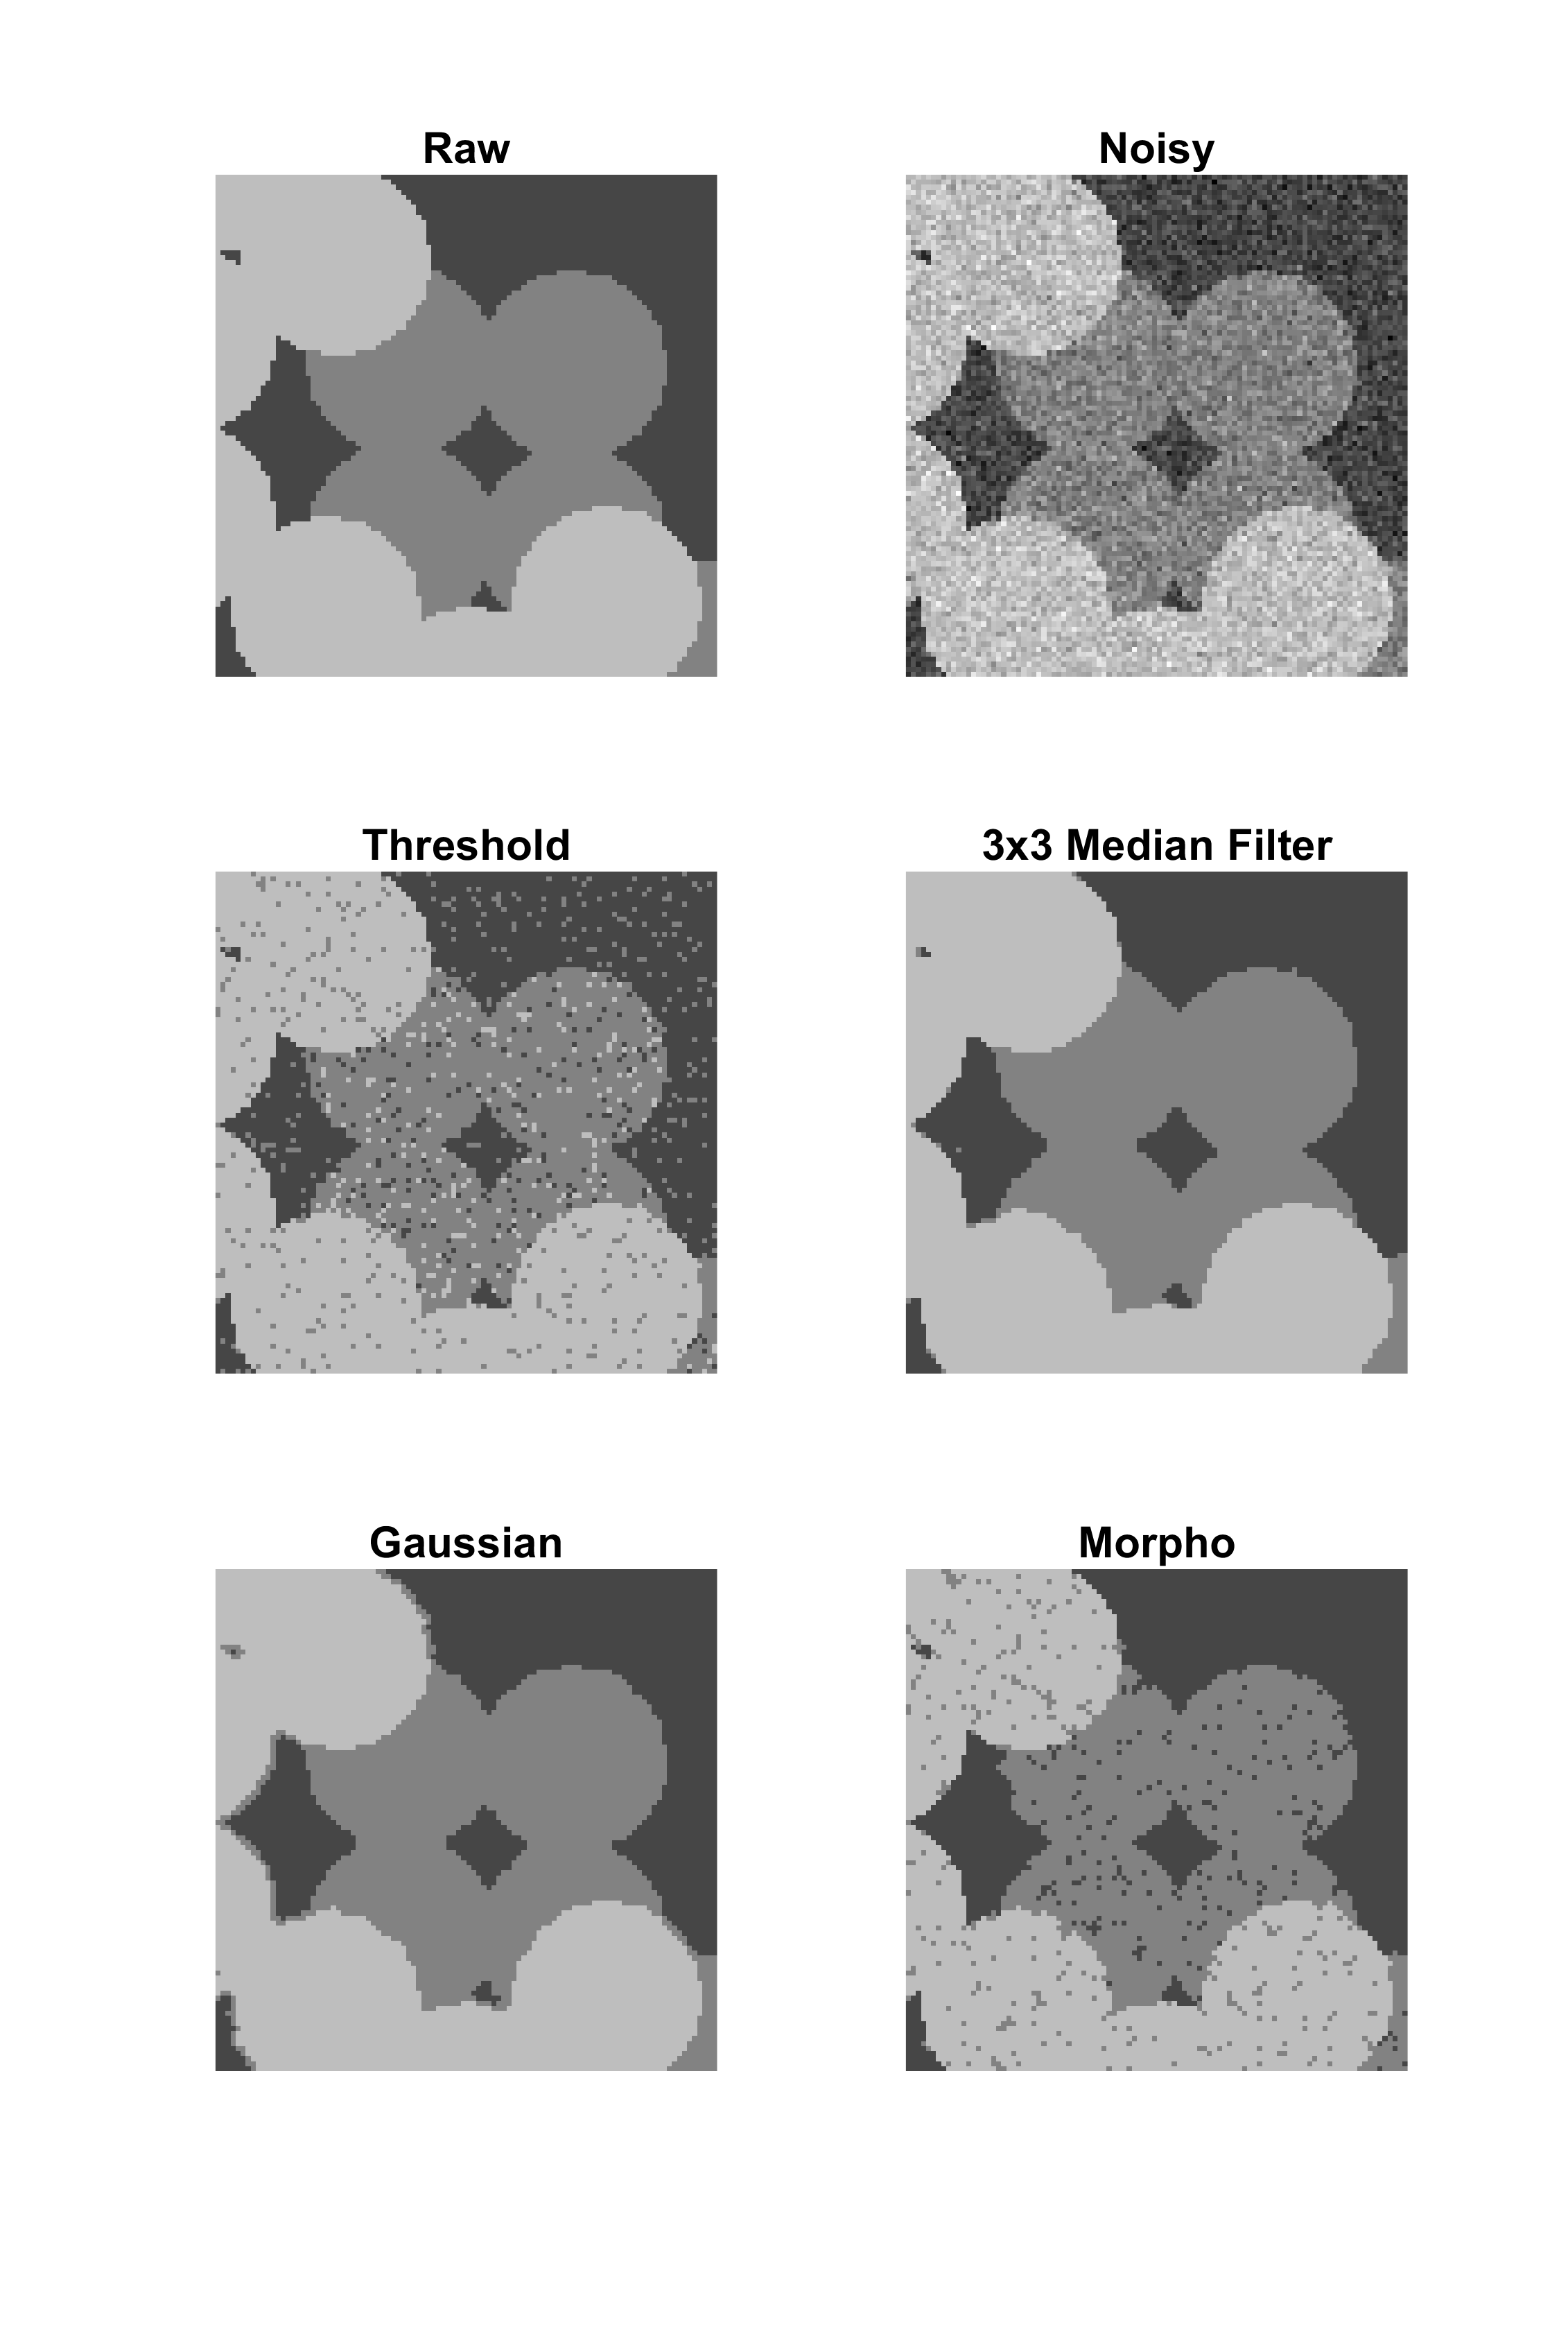
\includegraphics[width=0.54\textwidth]{./figures/res2.png}
	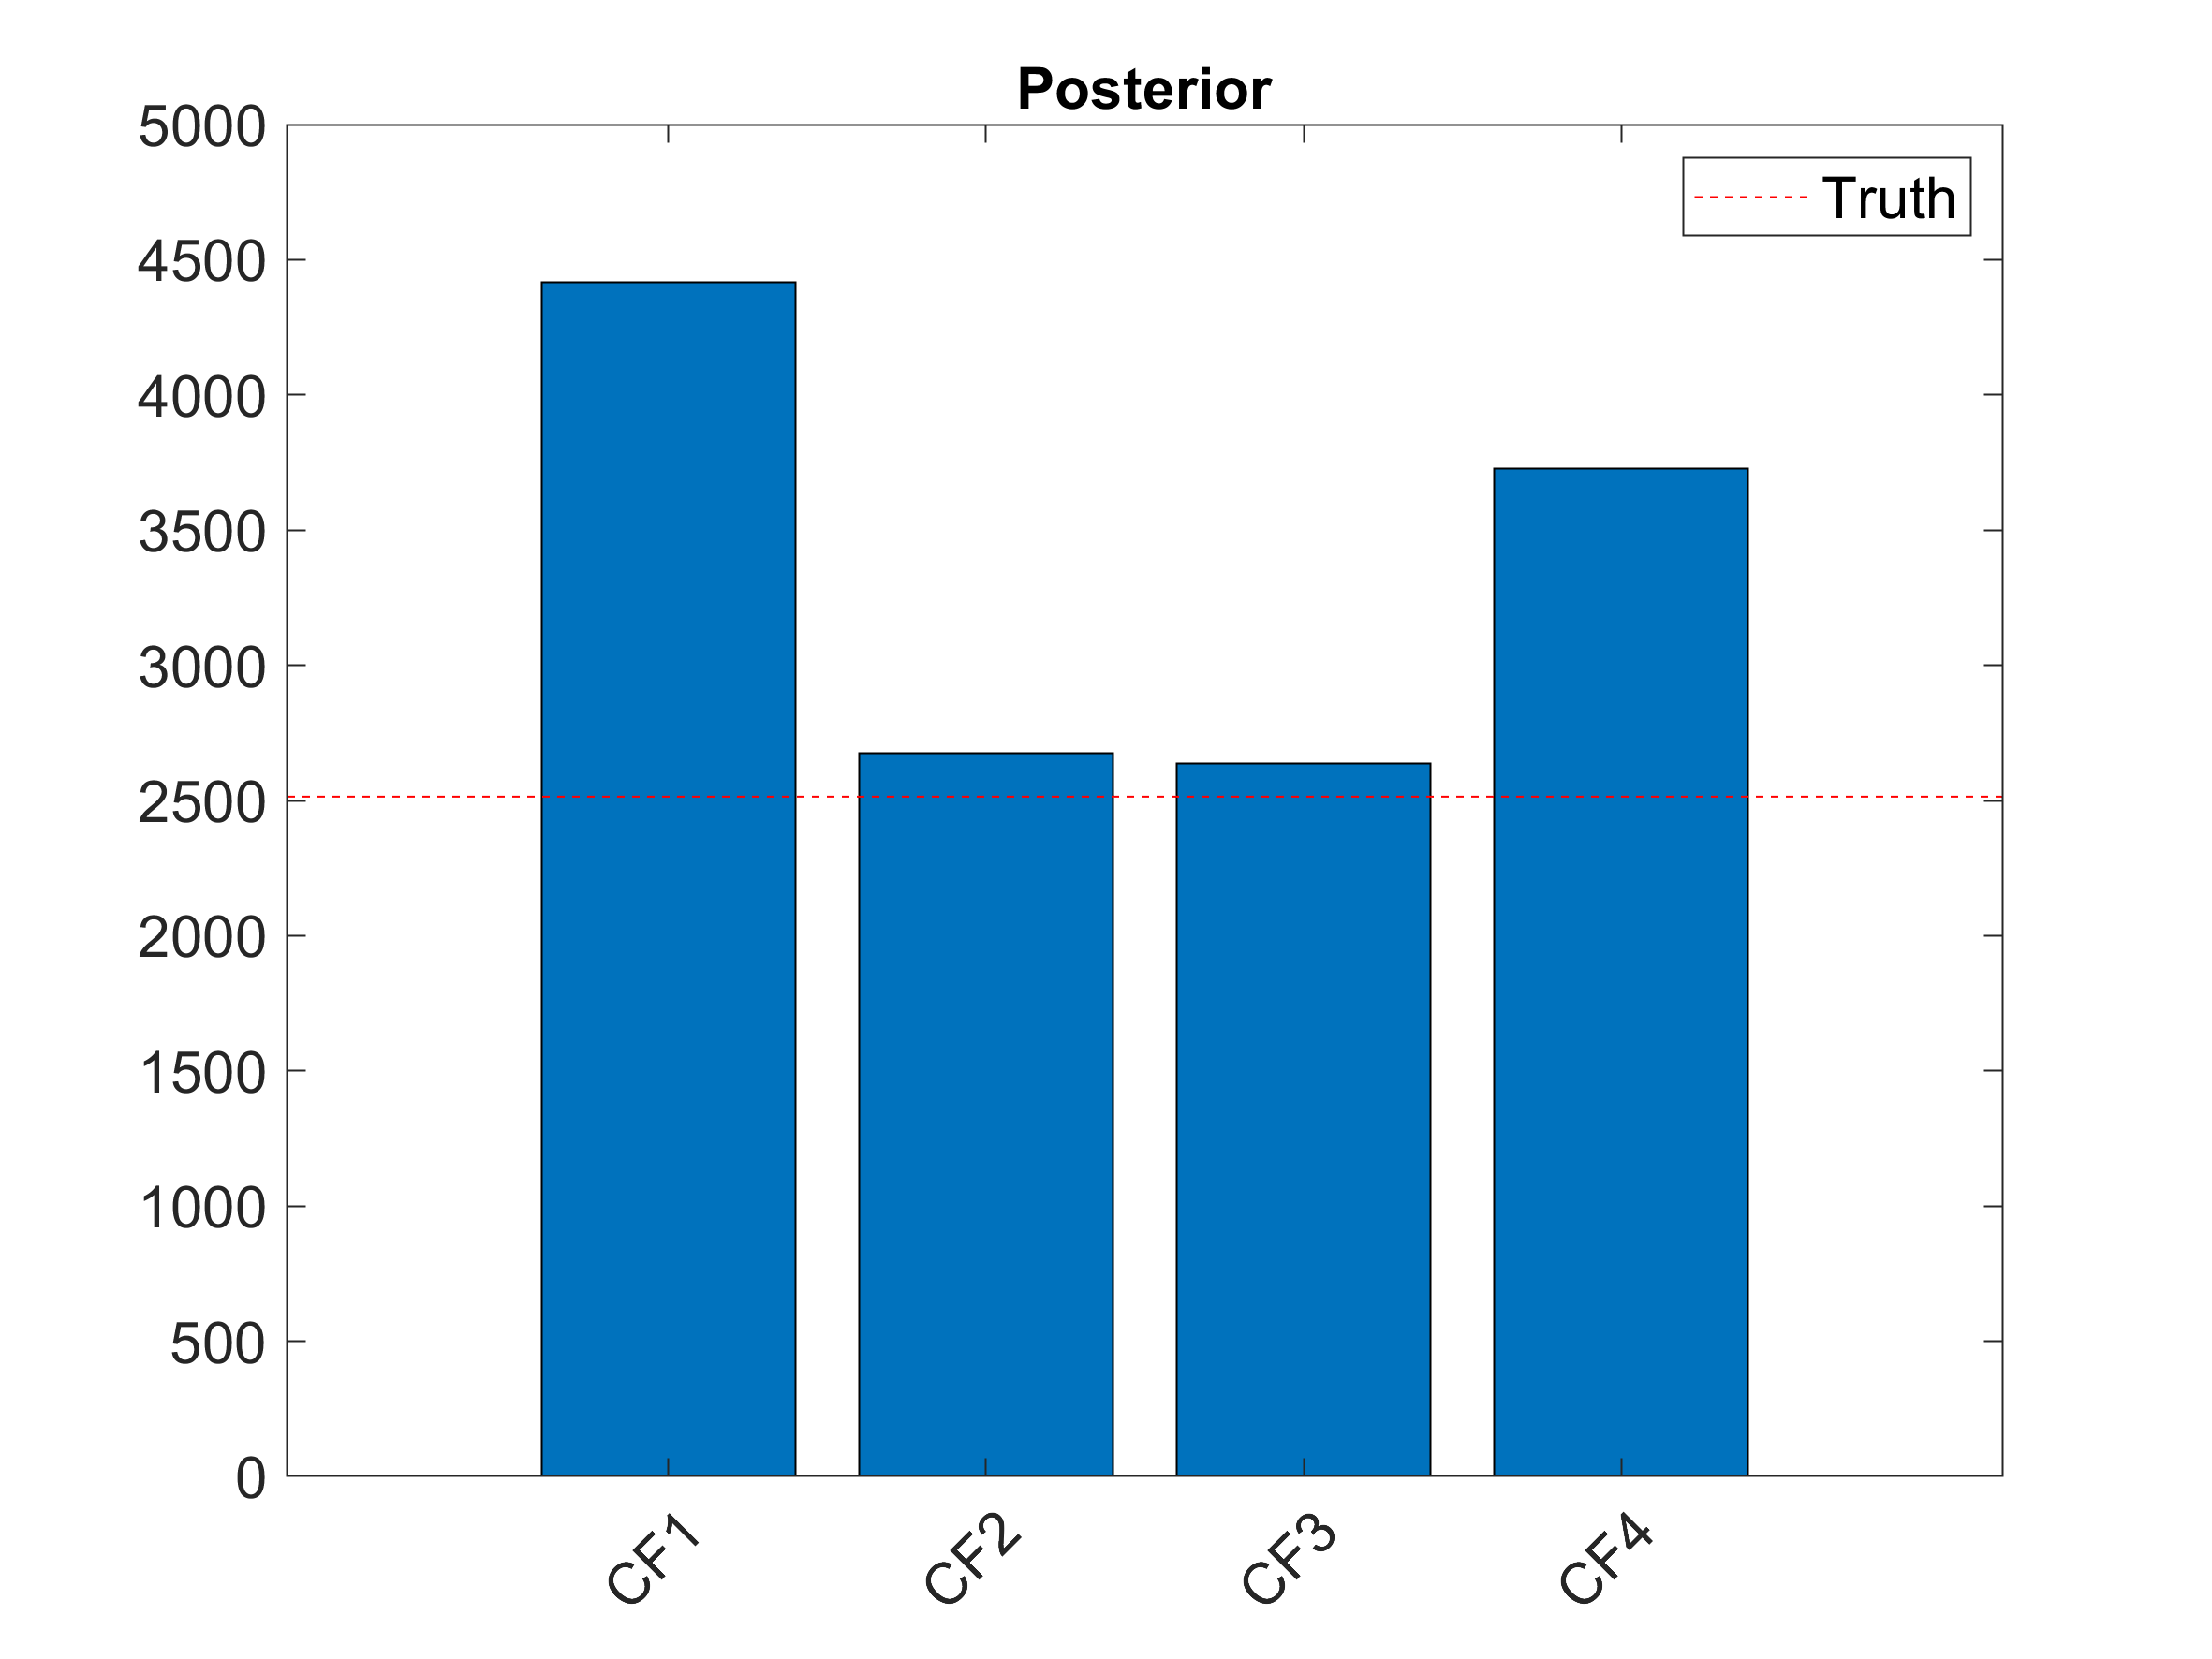
\includegraphics[width=0.45\textwidth]{./figures/res4.png}
    \caption{Left image shows the comparison of using four simple configurations. Visually speaking, the median filter based configuration can give us the best result. A guess would be that the added noise could be salty noise. The simple threshold cannot produce a promising result. However, it can be improved by applying a Gaussian filter in advance. The cost to pay it that the edges may be destroyed to some extent. The right image shows the cost comparison: it is clear that the median filter and Gaussian filter give the most approximated results compared with ground truth.}
\end{figure*}

	\begin{figure}[htbp]
	\centering
	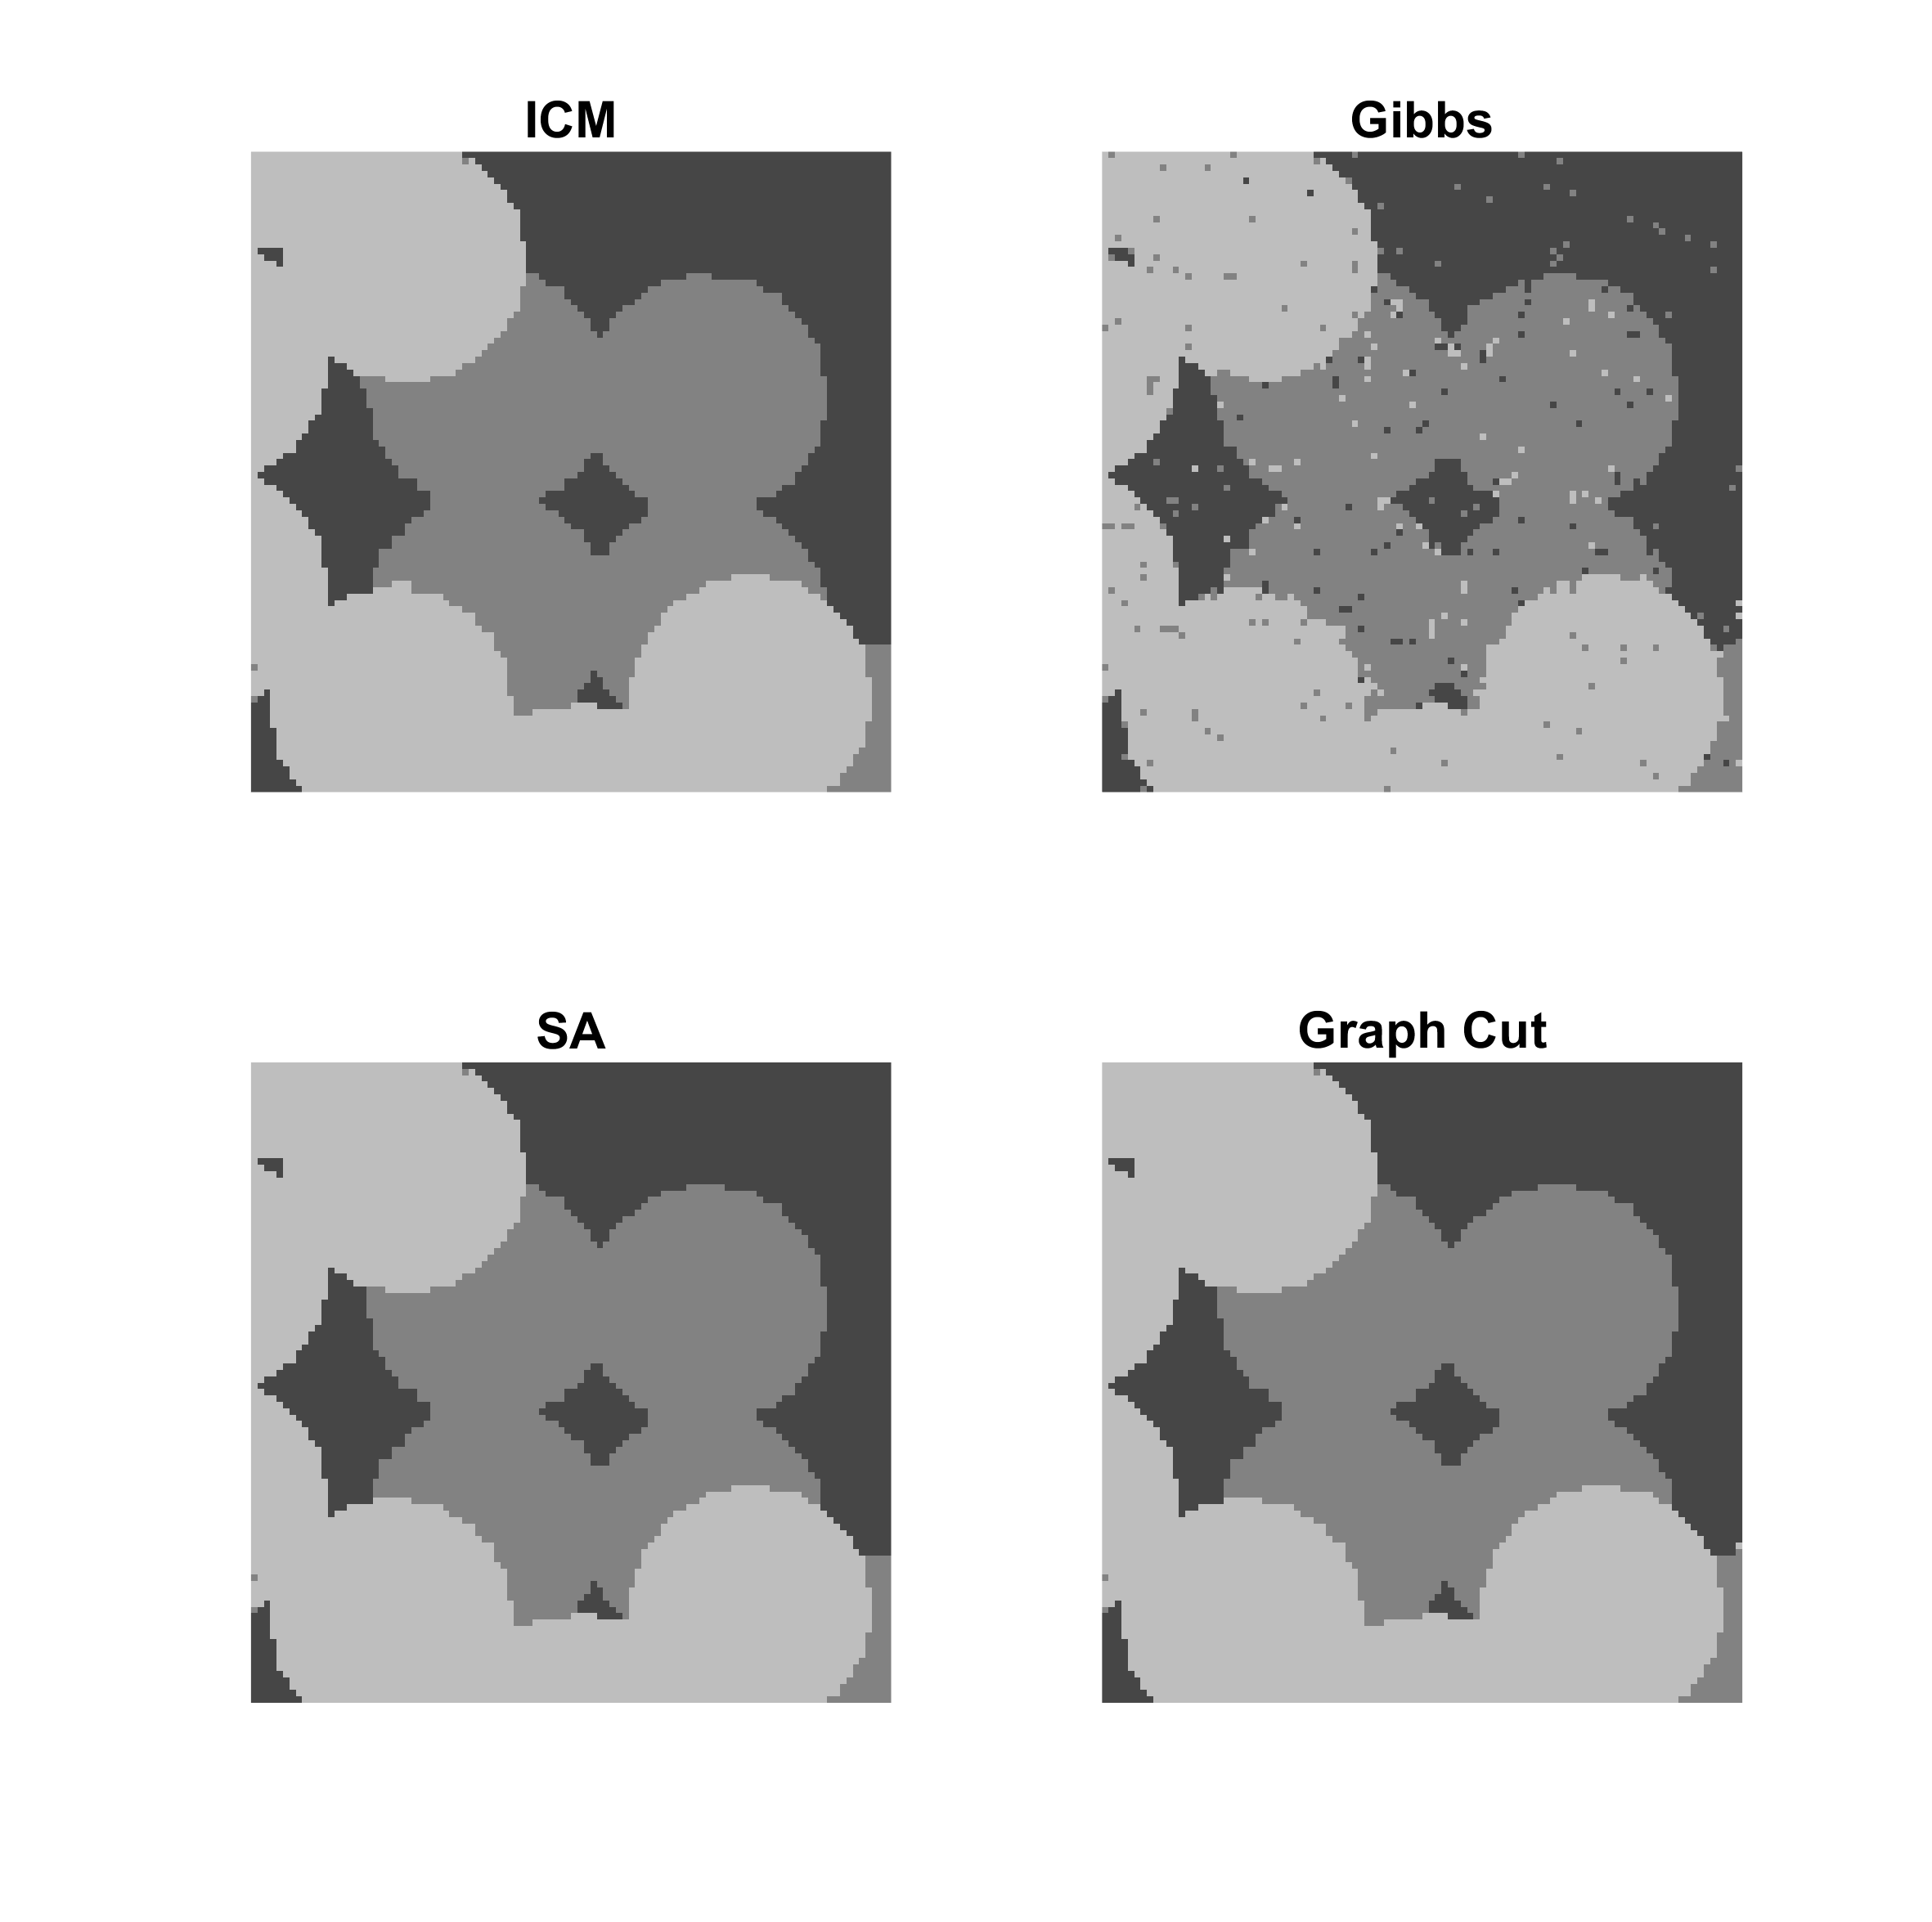
\includegraphics[width=0.6\textwidth]{./figures/cmp1.png}
	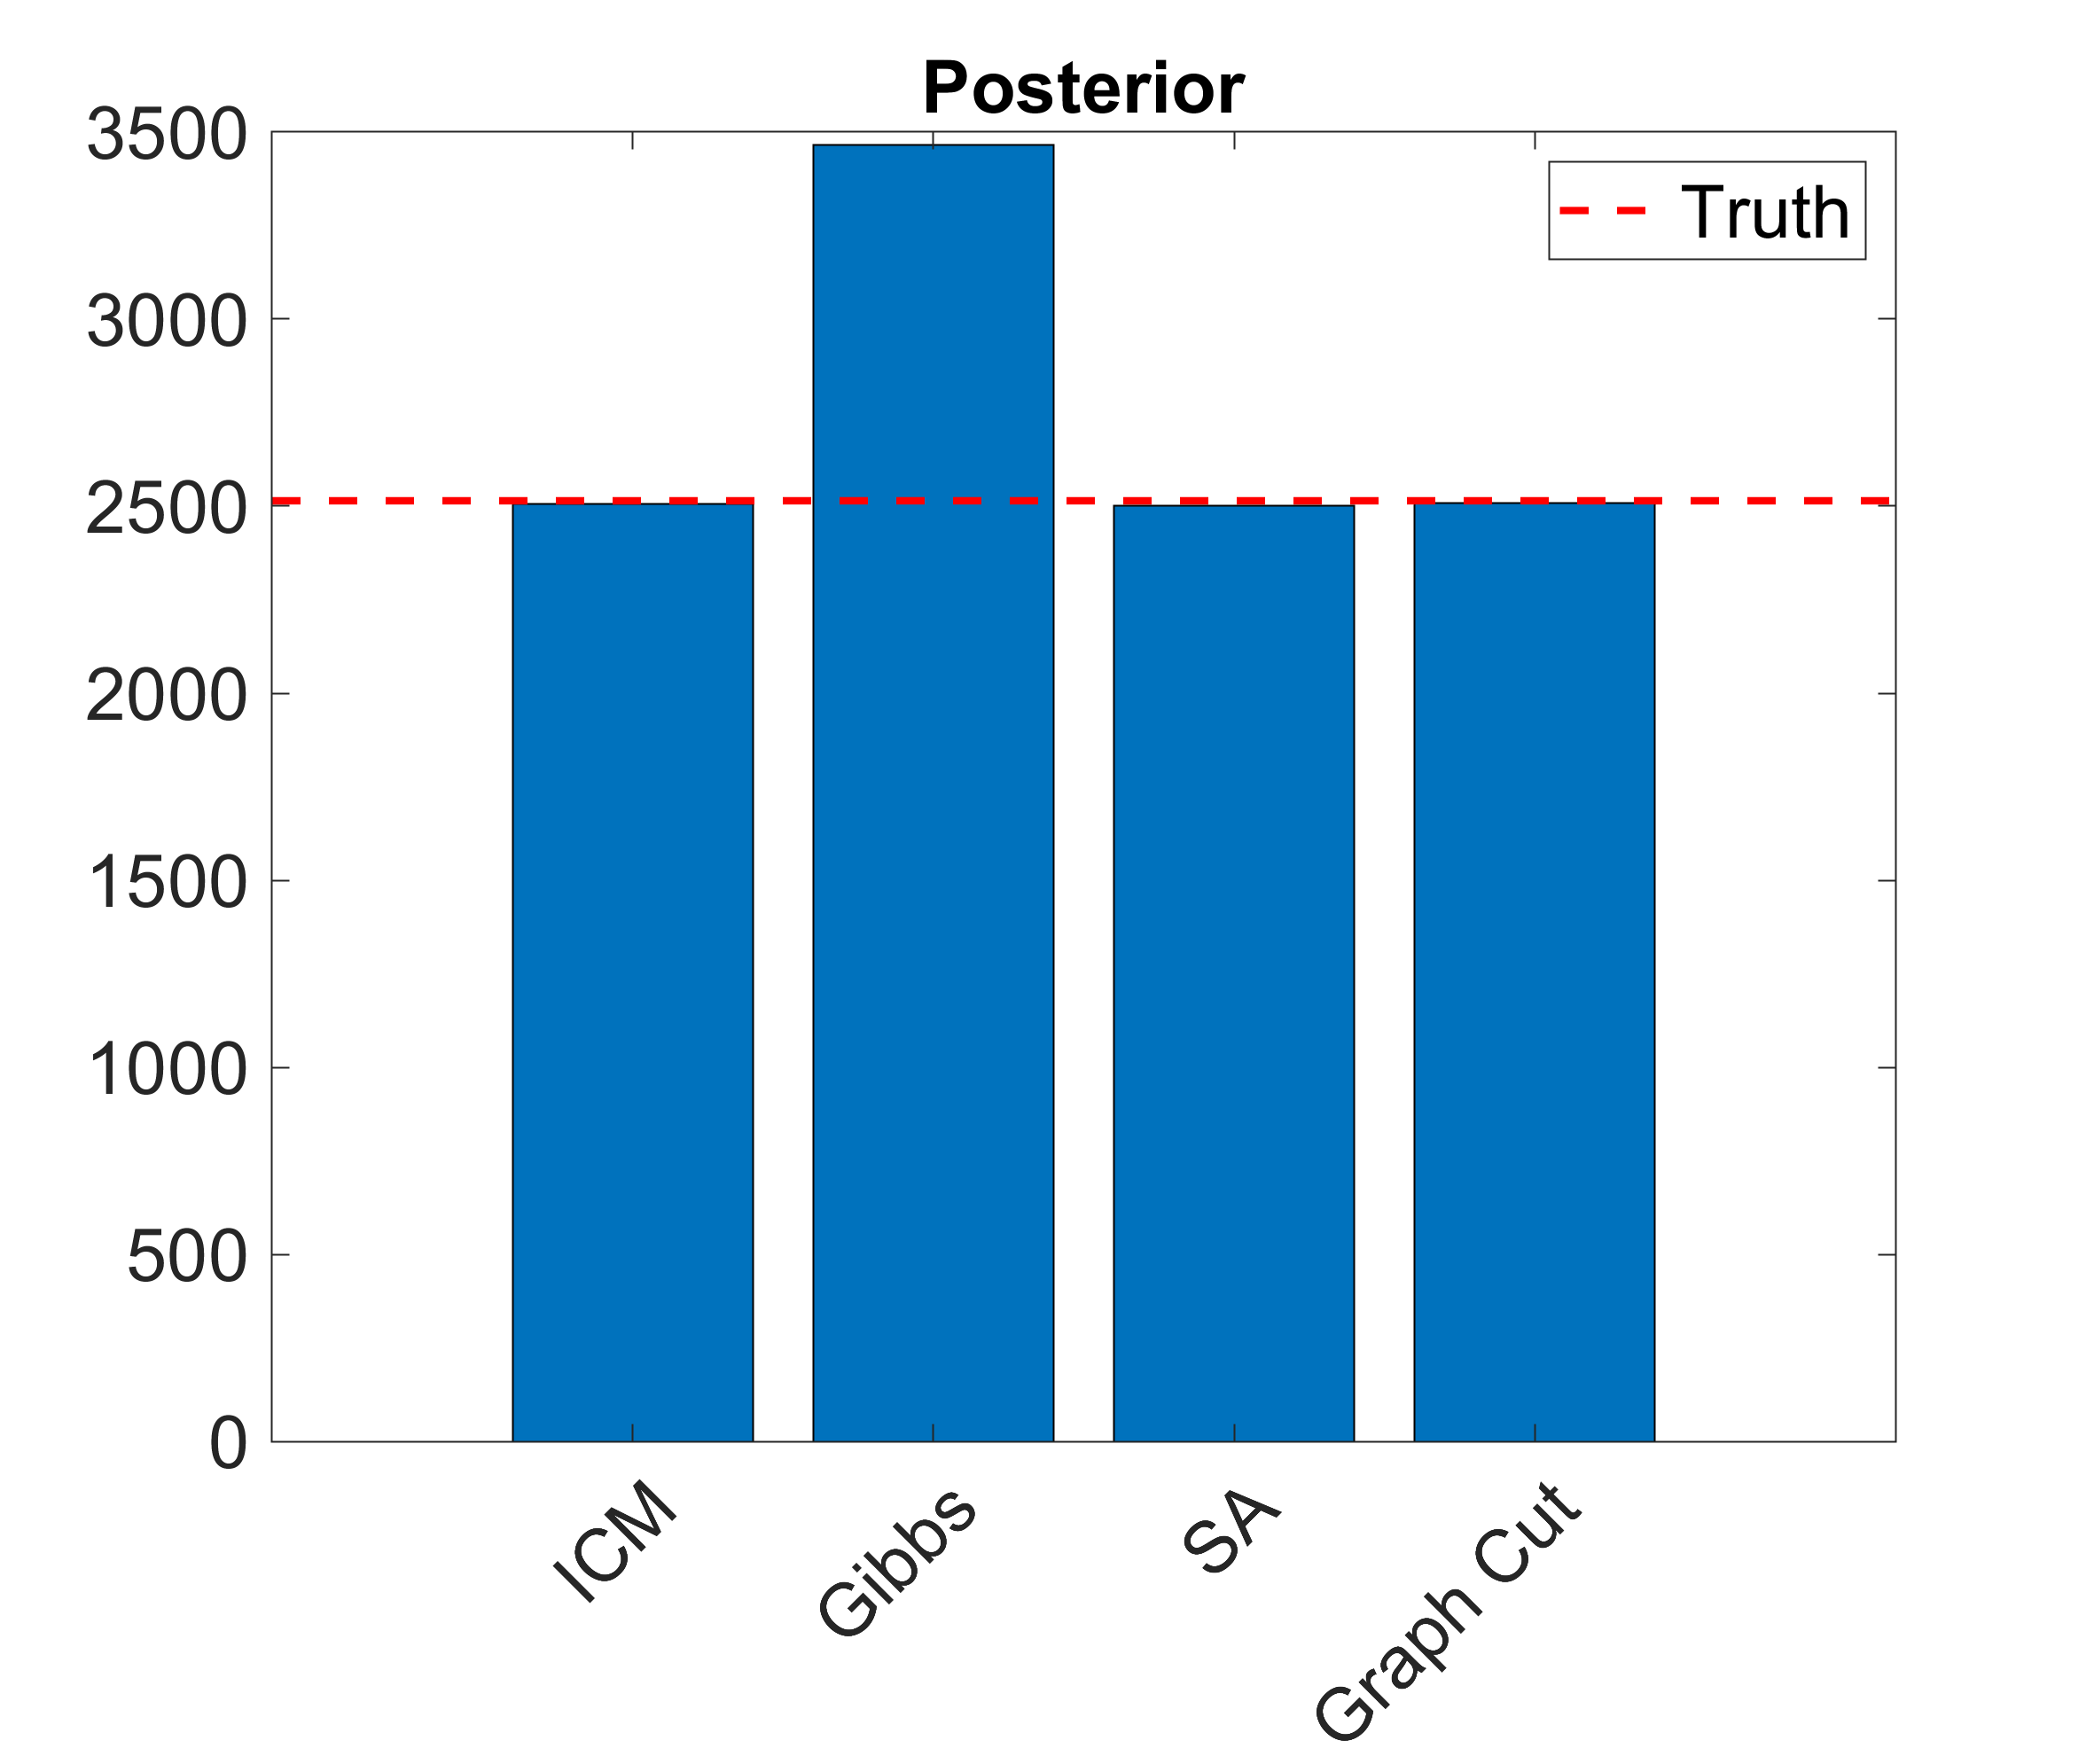
\includegraphics[width=0.38\textwidth]{./figures/cmp2.png}
    \caption{Comparison of using MRF with different optimization approaches. Visually speaking, ICM, Simulated Annealing, and Graph Cut give better performance than the Gibbs Sampling method. The right image shows the cost of the four optimization approaches. It is clear that ICM, SA, and Graph Cut all achieves the ground truth. However, local optimization method like ICM cannot always guarantee to achieve the global minimum. SA, however, is probabilistic optimum. So with the iteration increasing, its probability of achieving global optimum will increase up to 1. Graph cut is a globally optimal method for binary label segmentation.}
\end{figure}

	\begin{figure}[htbp]
	\centering
	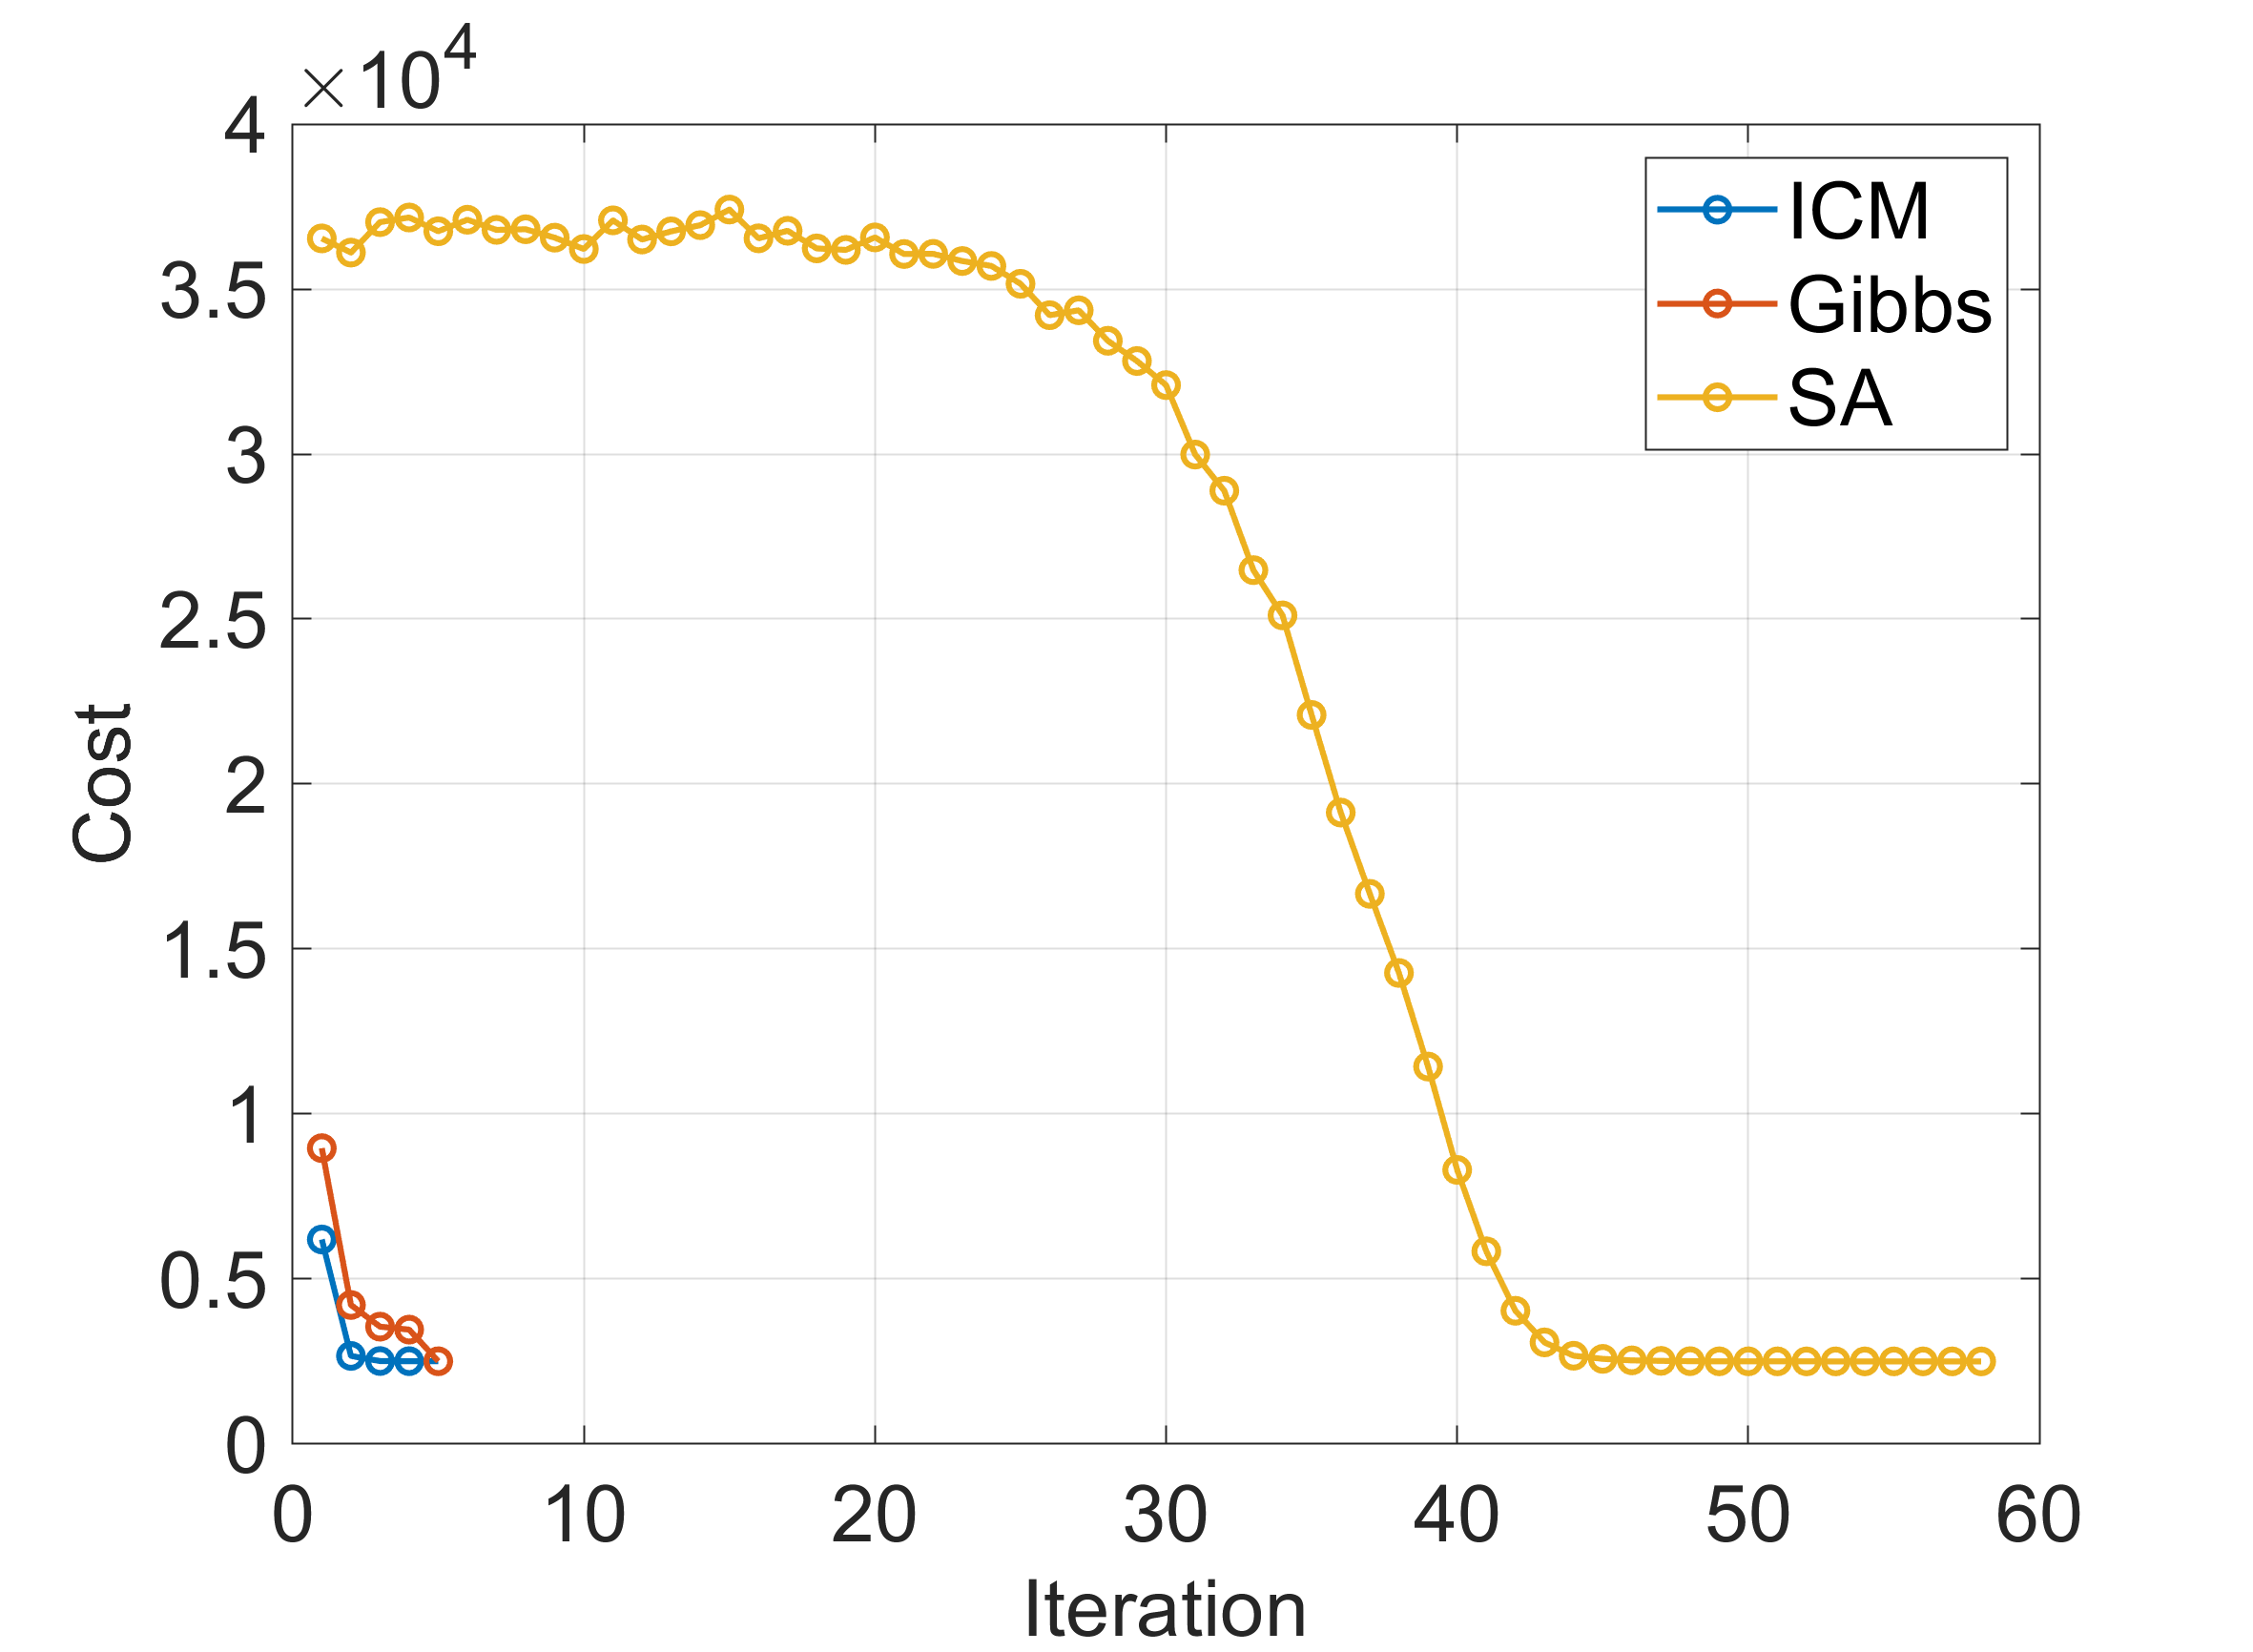
\includegraphics[width=0.5\textwidth]{./figures/cmp.png}
    \caption{Iteration comparison: SA will use more iteration to converge because it needs the temperature to be cooled down. Faster convergence can be achieved by make temperature cool down faster at the expense of increasing the possibility of being trapped in a local minimum. ICM and Gibbs sampling methods can converge rapidly compared with SA.}
\end{figure}

	\begin{figure}[htbp]
	\centering
	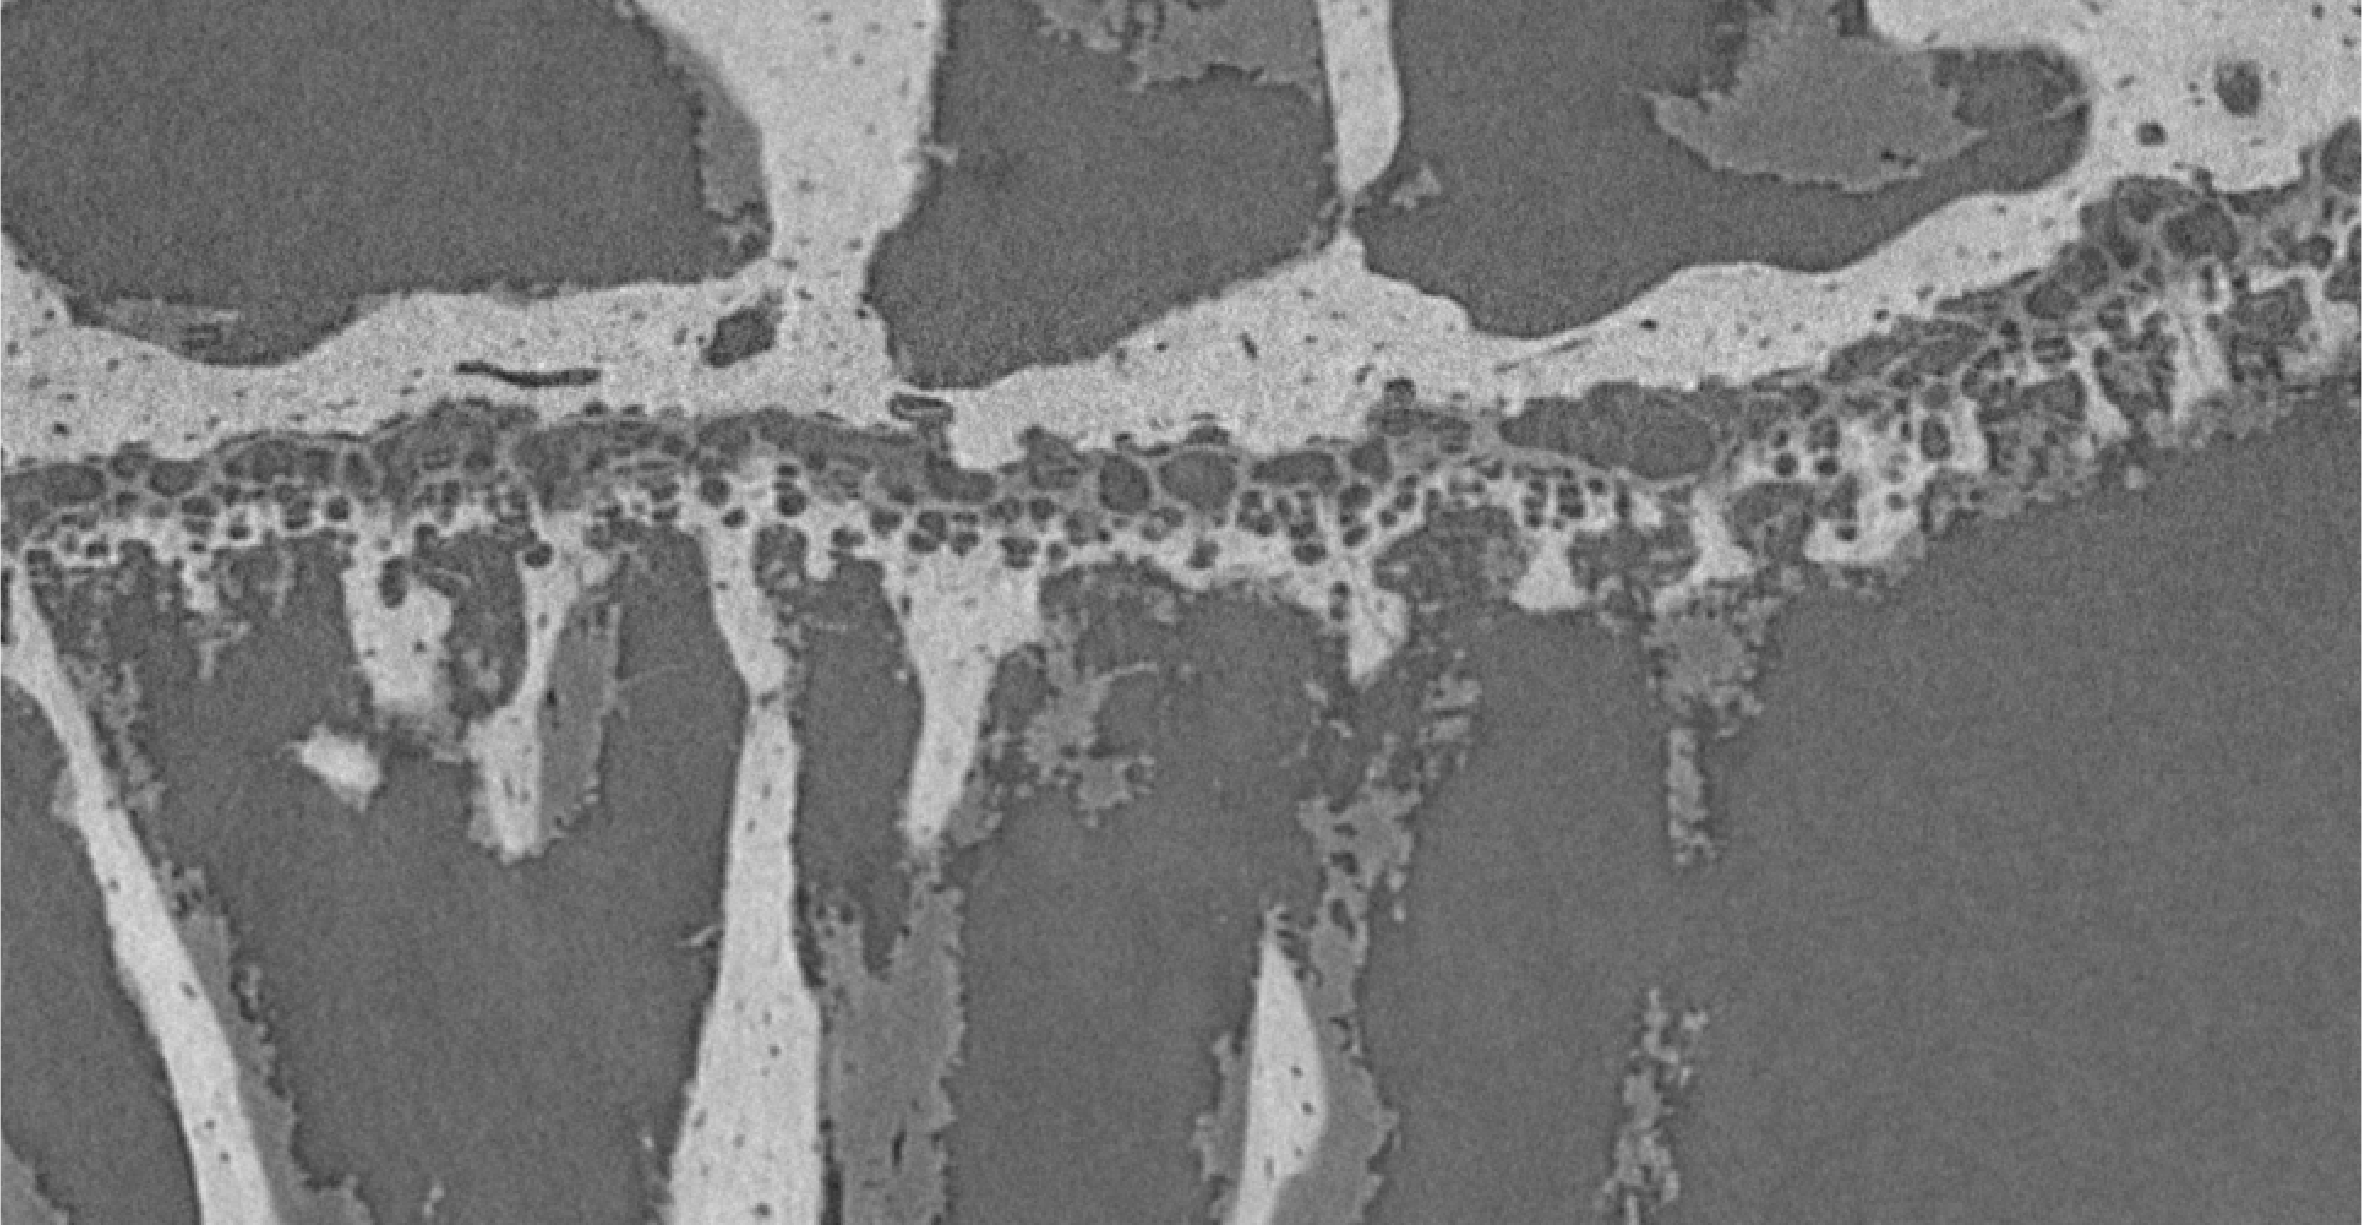
\includegraphics[width=0.5\textwidth]{./figures/assign2_raw.png}
	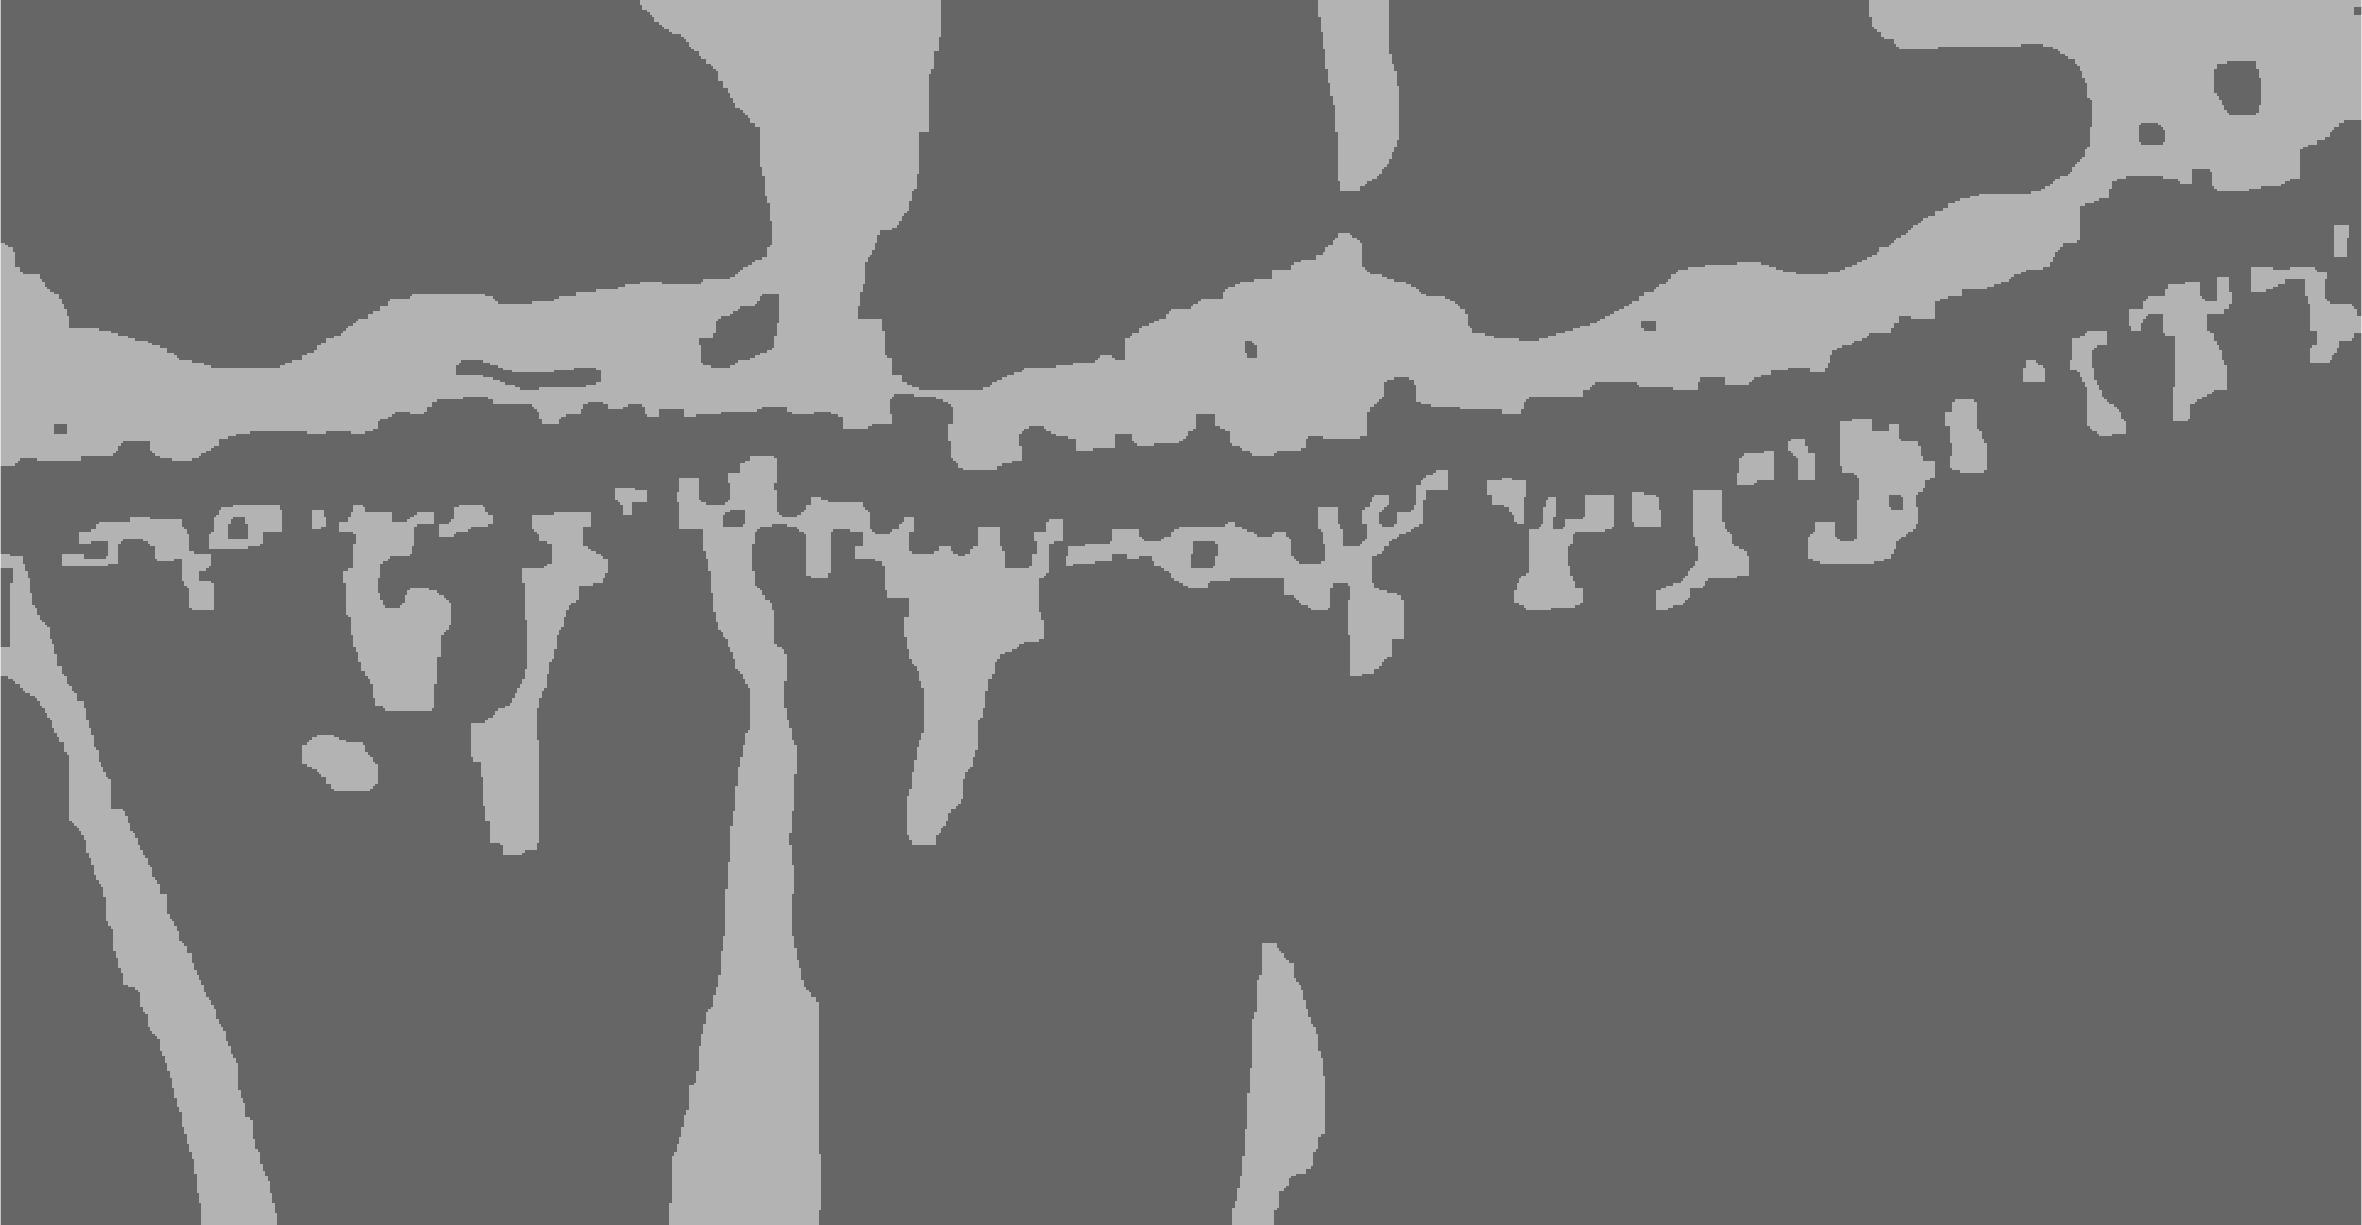
\includegraphics[width=0.5\textwidth]{./figures/assign2_seg.png}
	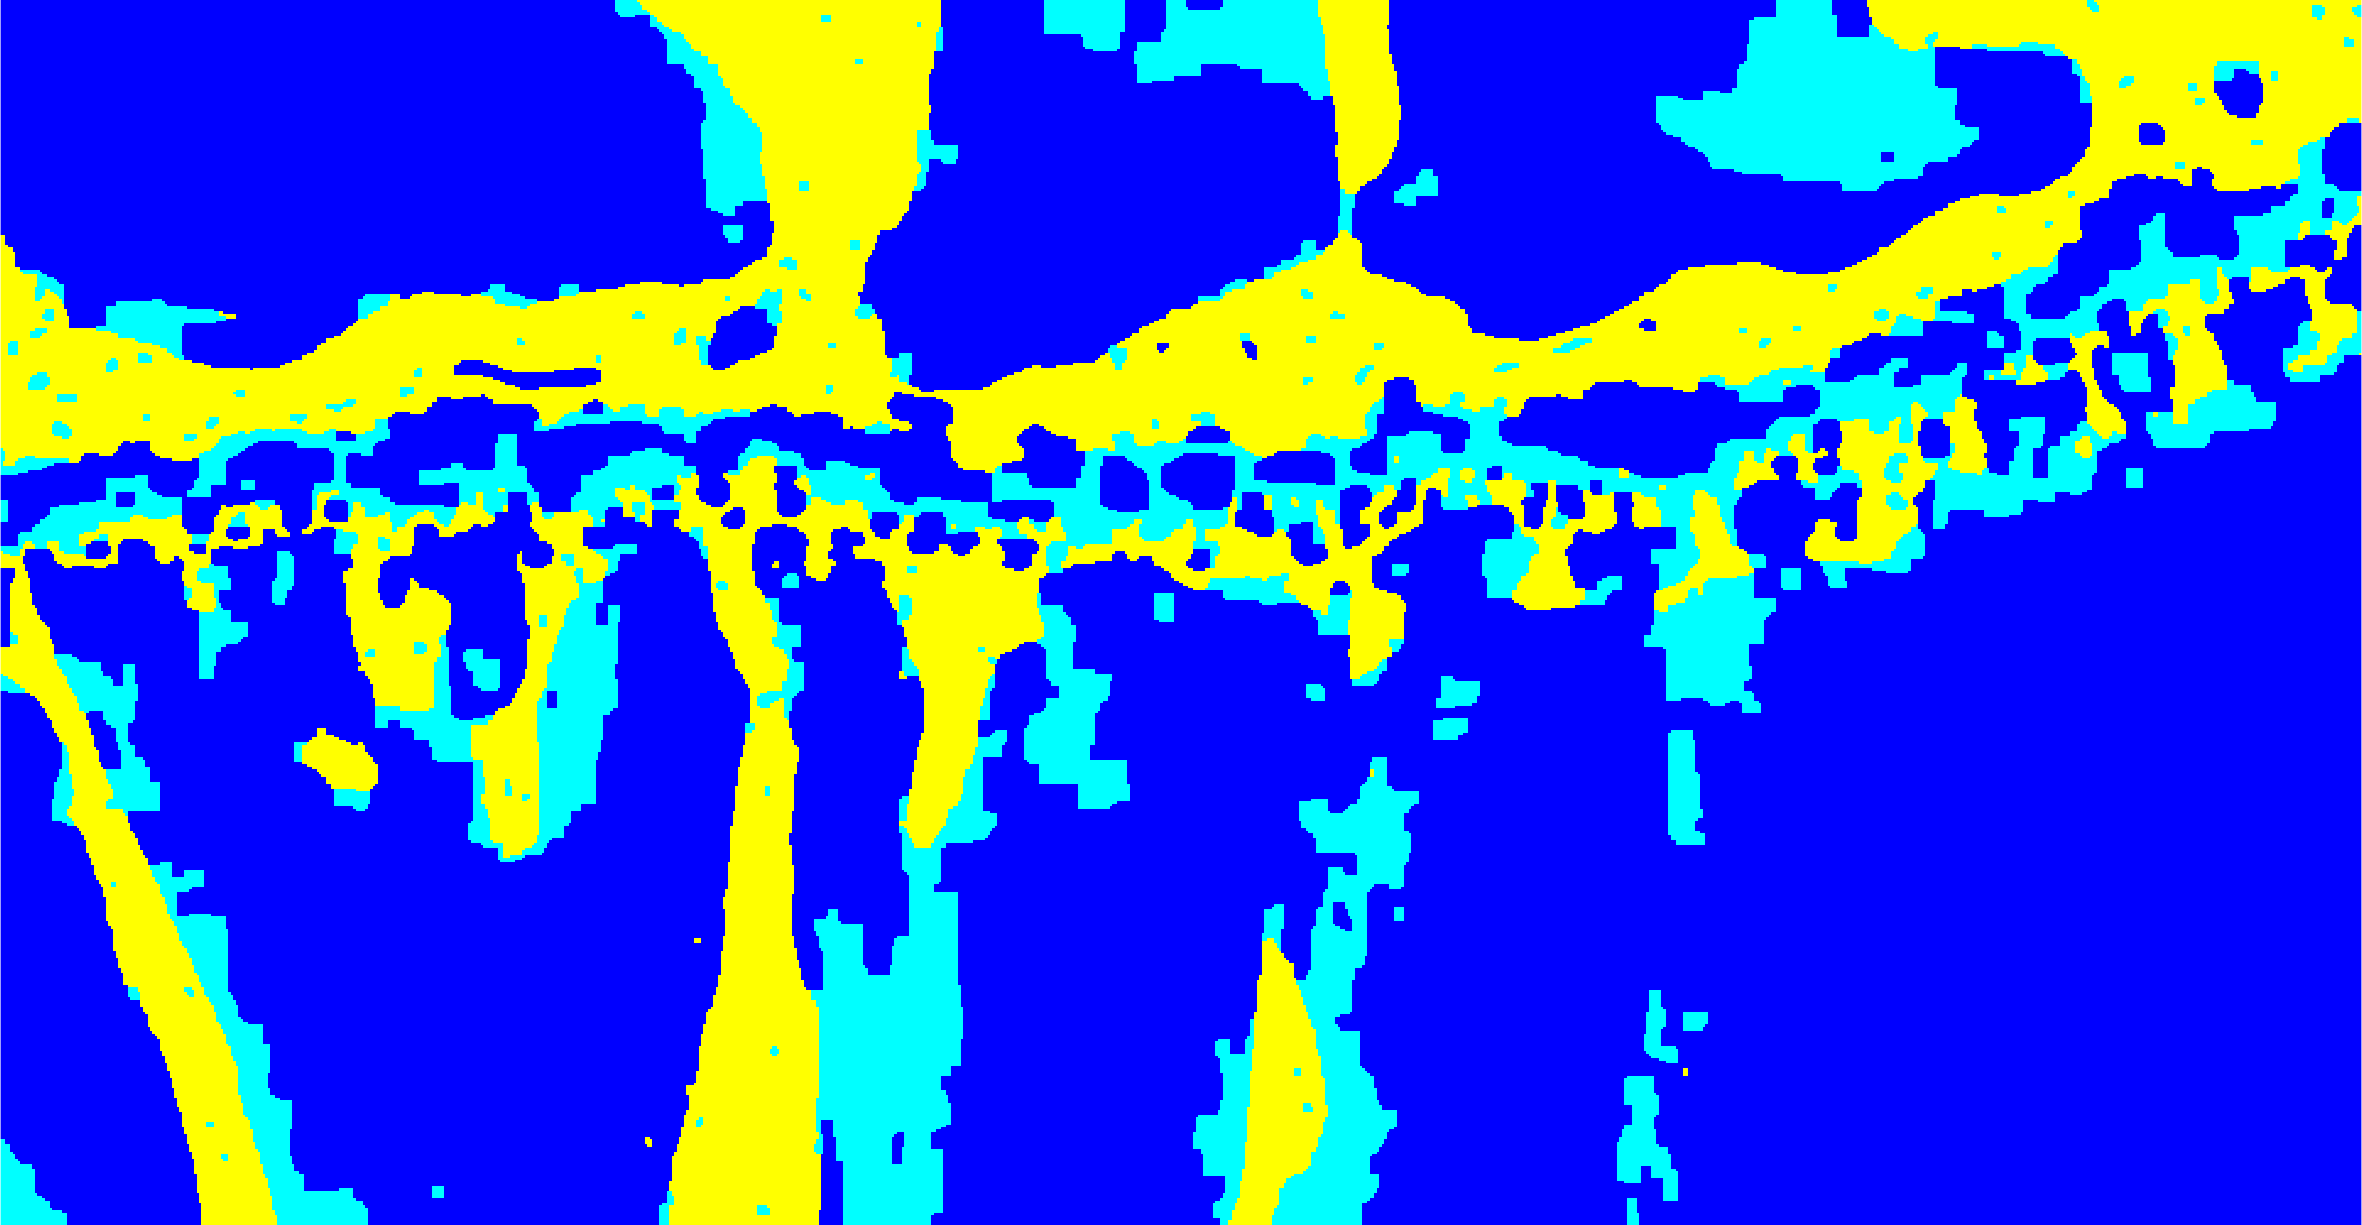
\includegraphics[width=0.5\textwidth]{./figures/assign2_mseg.png}
    \caption{Middle image shows the segmentation of bone (bright) and air (dark). The bottom image shows the segmentation of bone (yellow), cartilage (light blue), and air (dark blue).}
\end{figure}
	\section{Deformable Models}
	\begin{figure}[htbp]
	\centering
	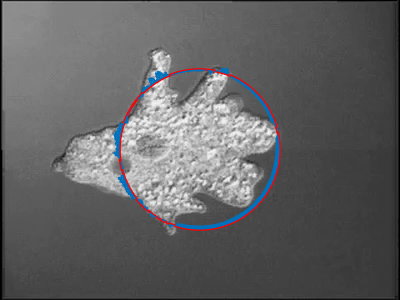
\includegraphics[width=0.45\textwidth]{./figures/defom1.png}
	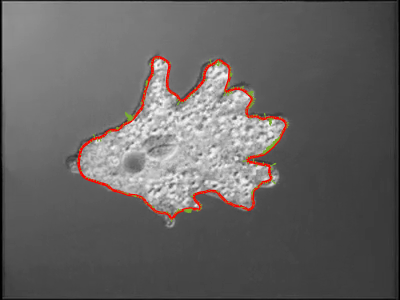
\includegraphics[width=0.45\textwidth]{./figures/defom2.png}
	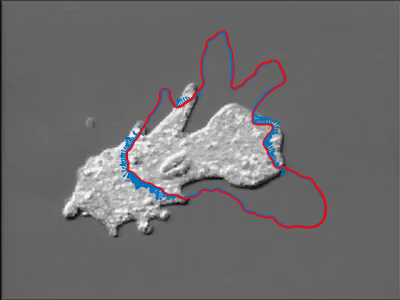
\includegraphics[width=0.45\textwidth]{./figures/defom148.png}
	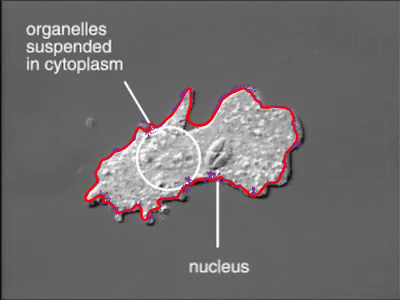
\includegraphics[width=0.45\textwidth]{./figures/defom186.png}
	\caption{Deformable models: top-left is the initial curve, the other three shows the intermediate results.}
\end{figure}
	\section{Geometric Priors}
	Several approaches have been applied for myelinated nerves segmentation, including:
	\begin{enumerate}
	\item Perform MRF segmentation slice by slice. This is done by firstly investigating the histogram of several sample images, and then perform MRF for binary segmentation. Parameters need to be finely tuned in order to have very good results. A snapshot of the final result is shown in Figure~\ref{final1}.
	\begin{figure}[!b]
	\centering
	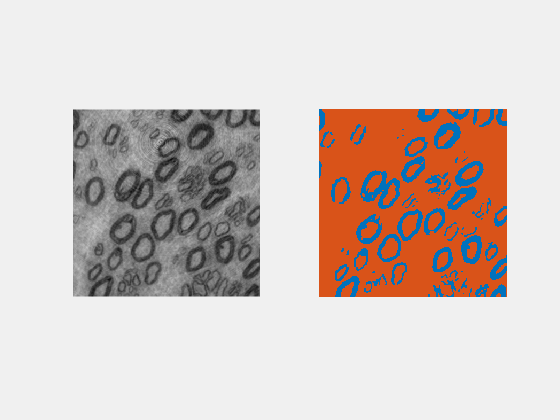
\includegraphics[width=0.8\textwidth]{./figures/1.png}
	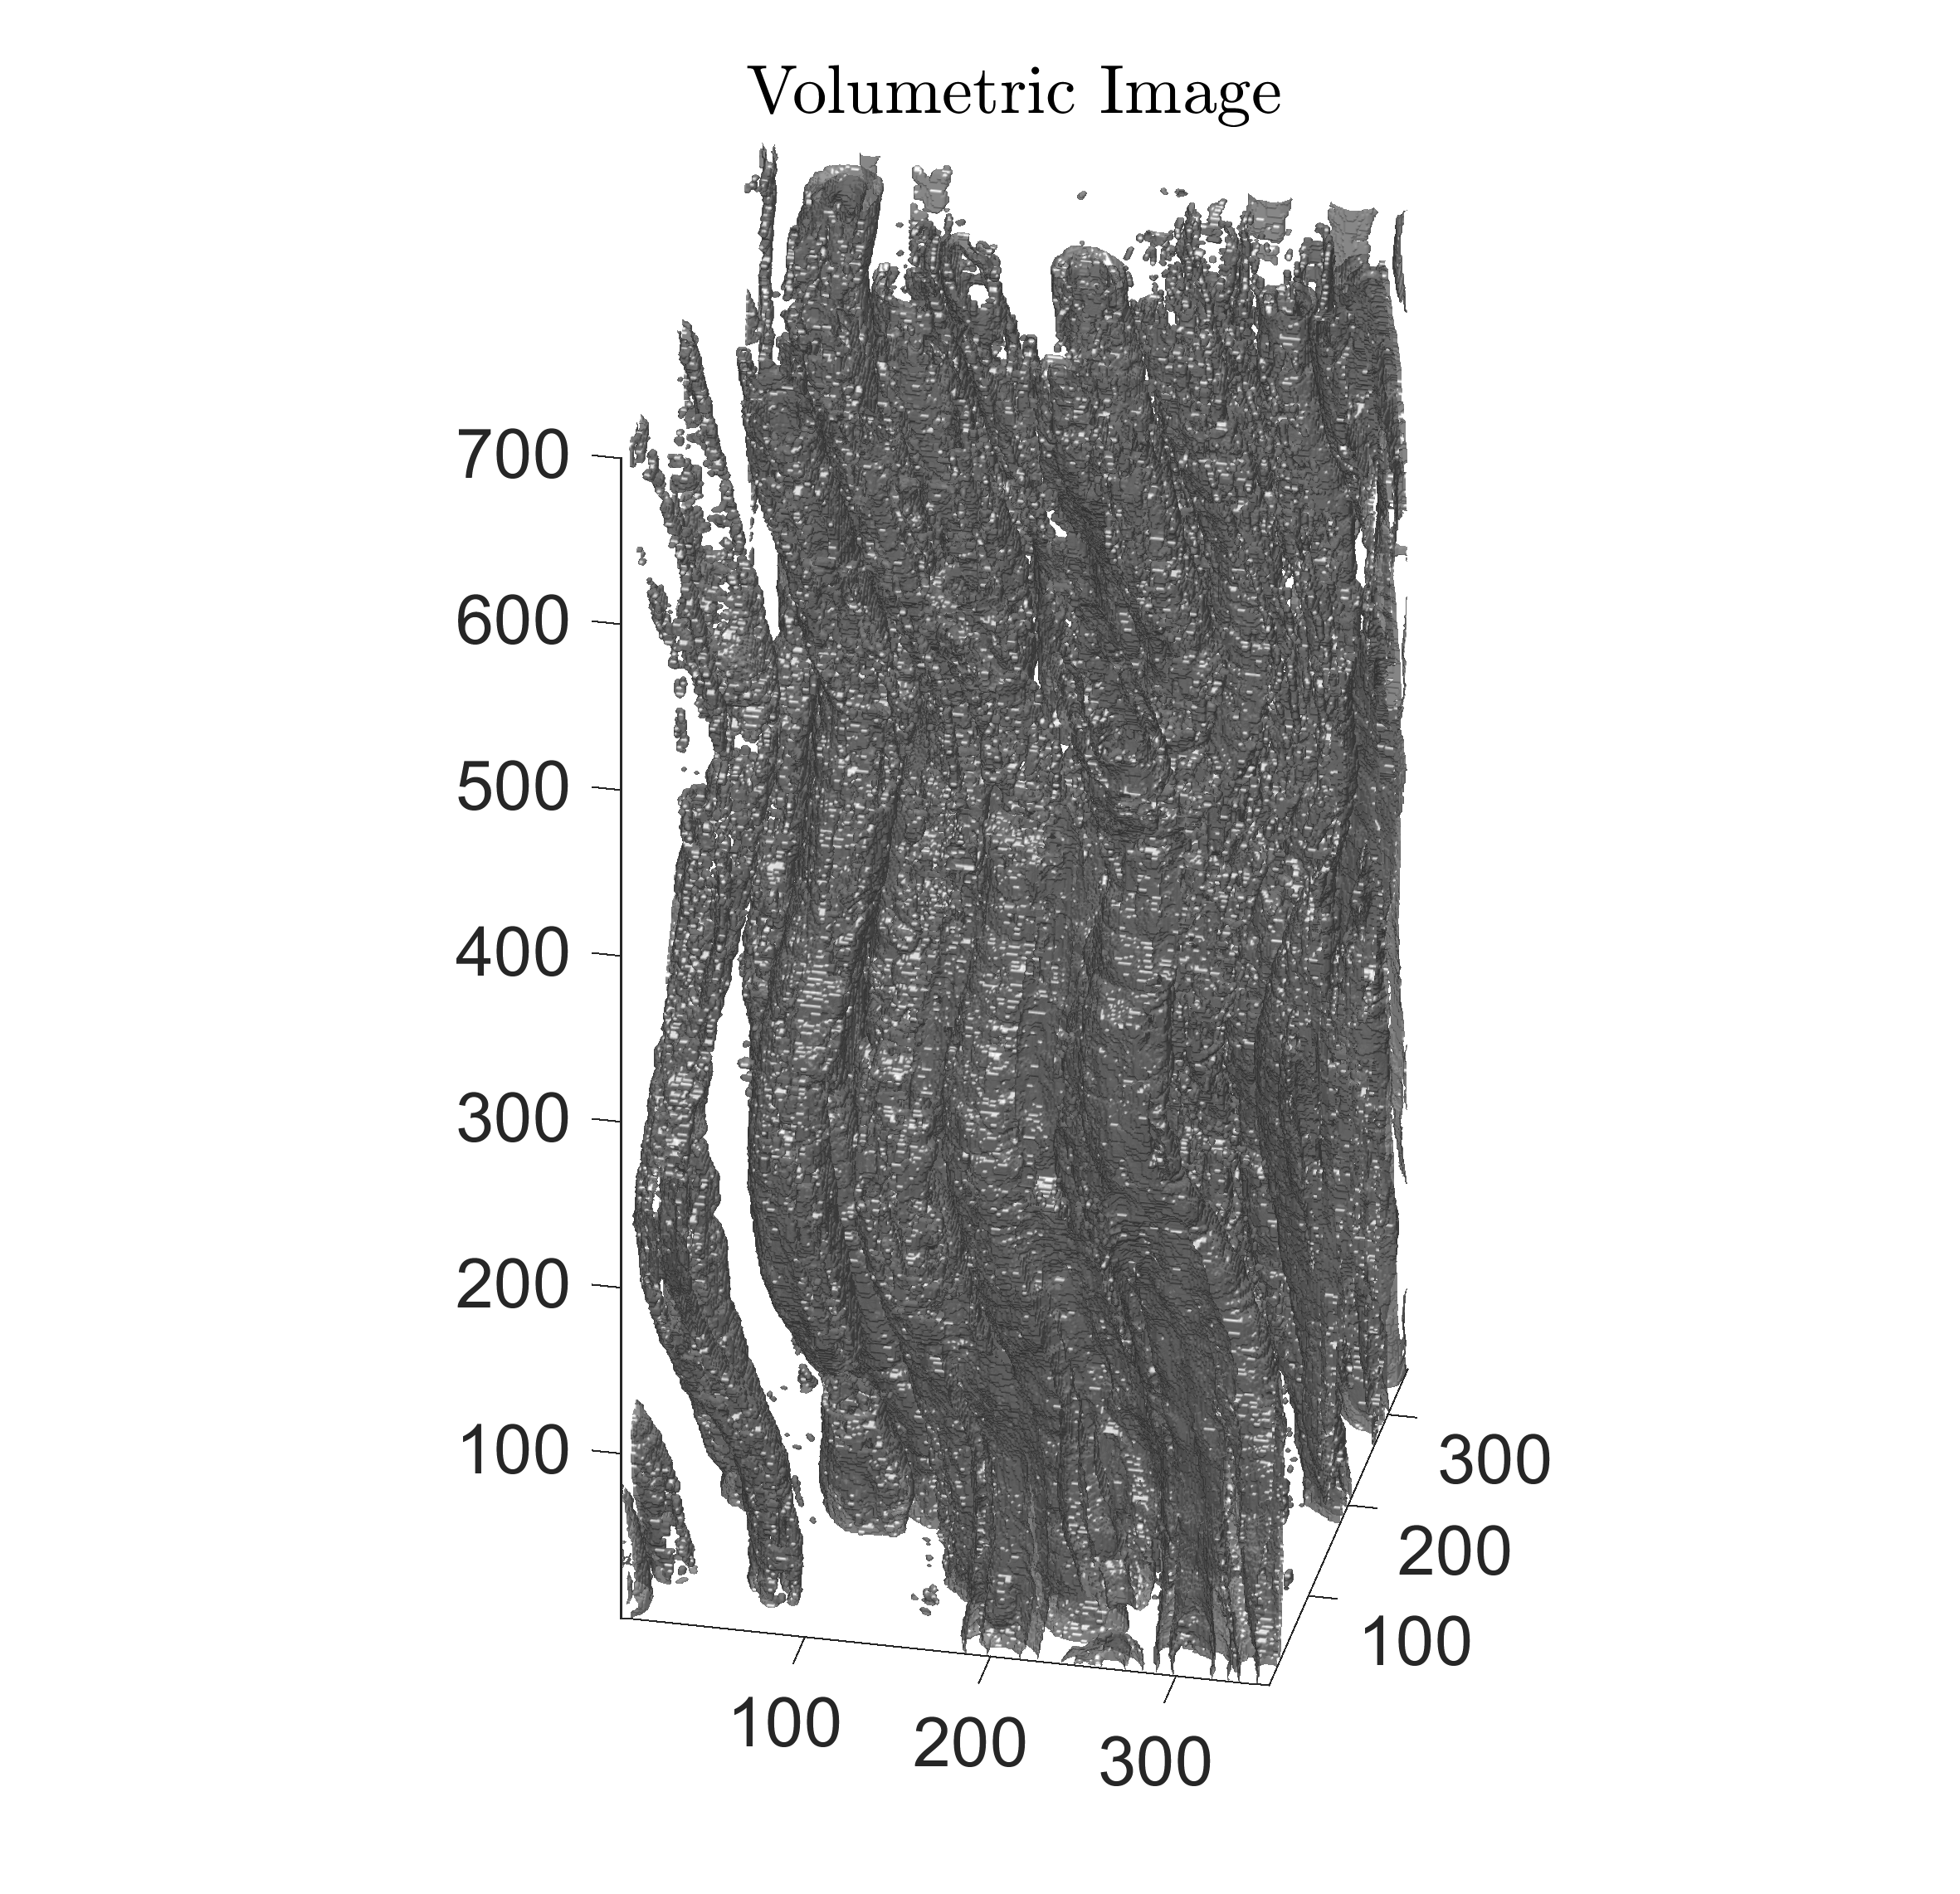
\includegraphics[width=0.8\textwidth]{./figures/final_res1.png}
    \caption{Top image is a snapshot of the slice-by-slice MRF segmentation of nerves image. The bottom image shows the 3D visualization of the segmented nerves.}
	\label{final1}
\end{figure}
	
	\item Perform MRF by considering smoothness among consecutive frames. Theoretically, it is possible to create a full 3D segmentation by stacking all images together. However, because of the memory constraint as well as for saving time, what I did in this assignment is to do the 3D segmentation using $100$ continuous images, i.e. $1-100$ as a batch, $101-200$ as the second batch. A snapshot of the final result is shown in Figure~\ref{final2}.
	
	\begin{figure}[!b]
	\centering
	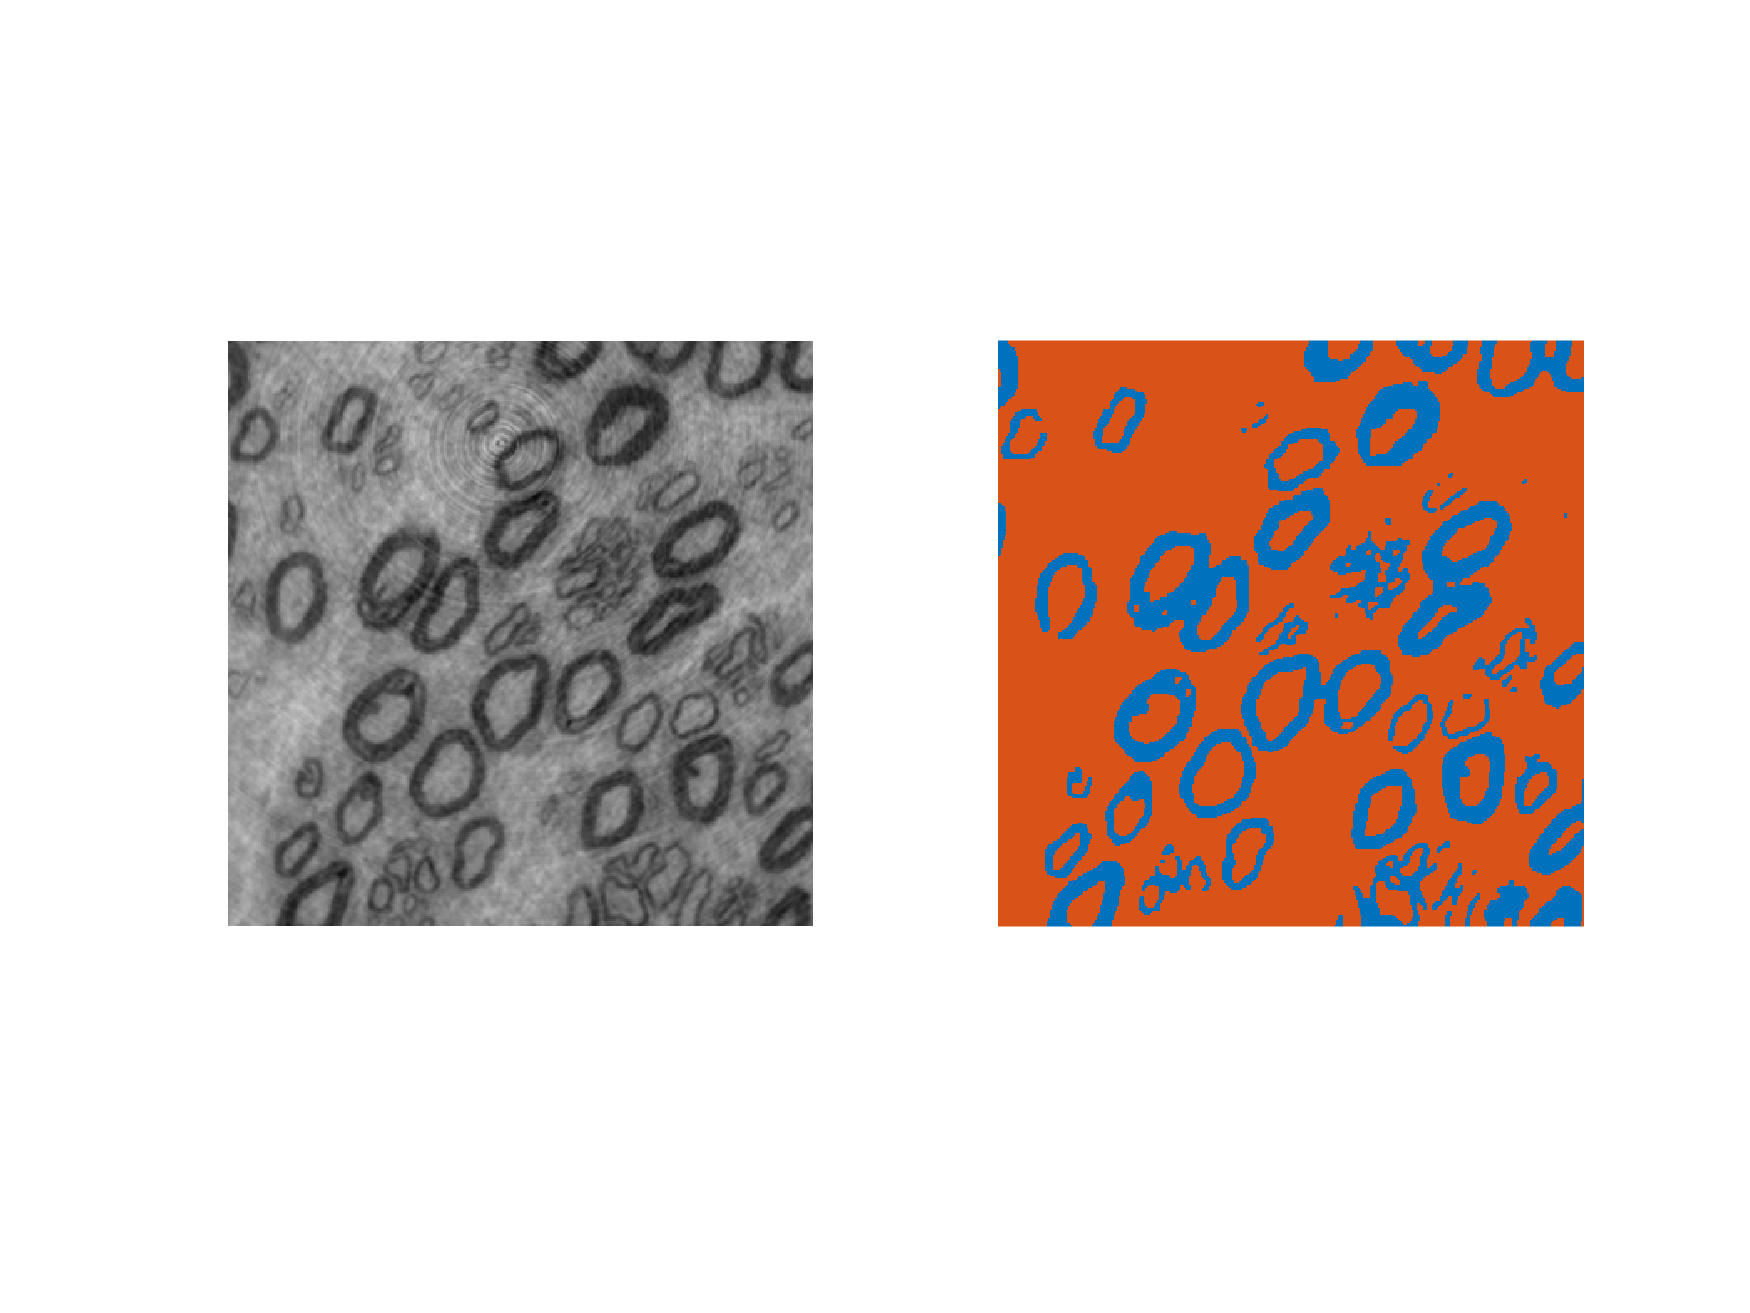
\includegraphics[width=0.8\textwidth]{./figures/2.png}
	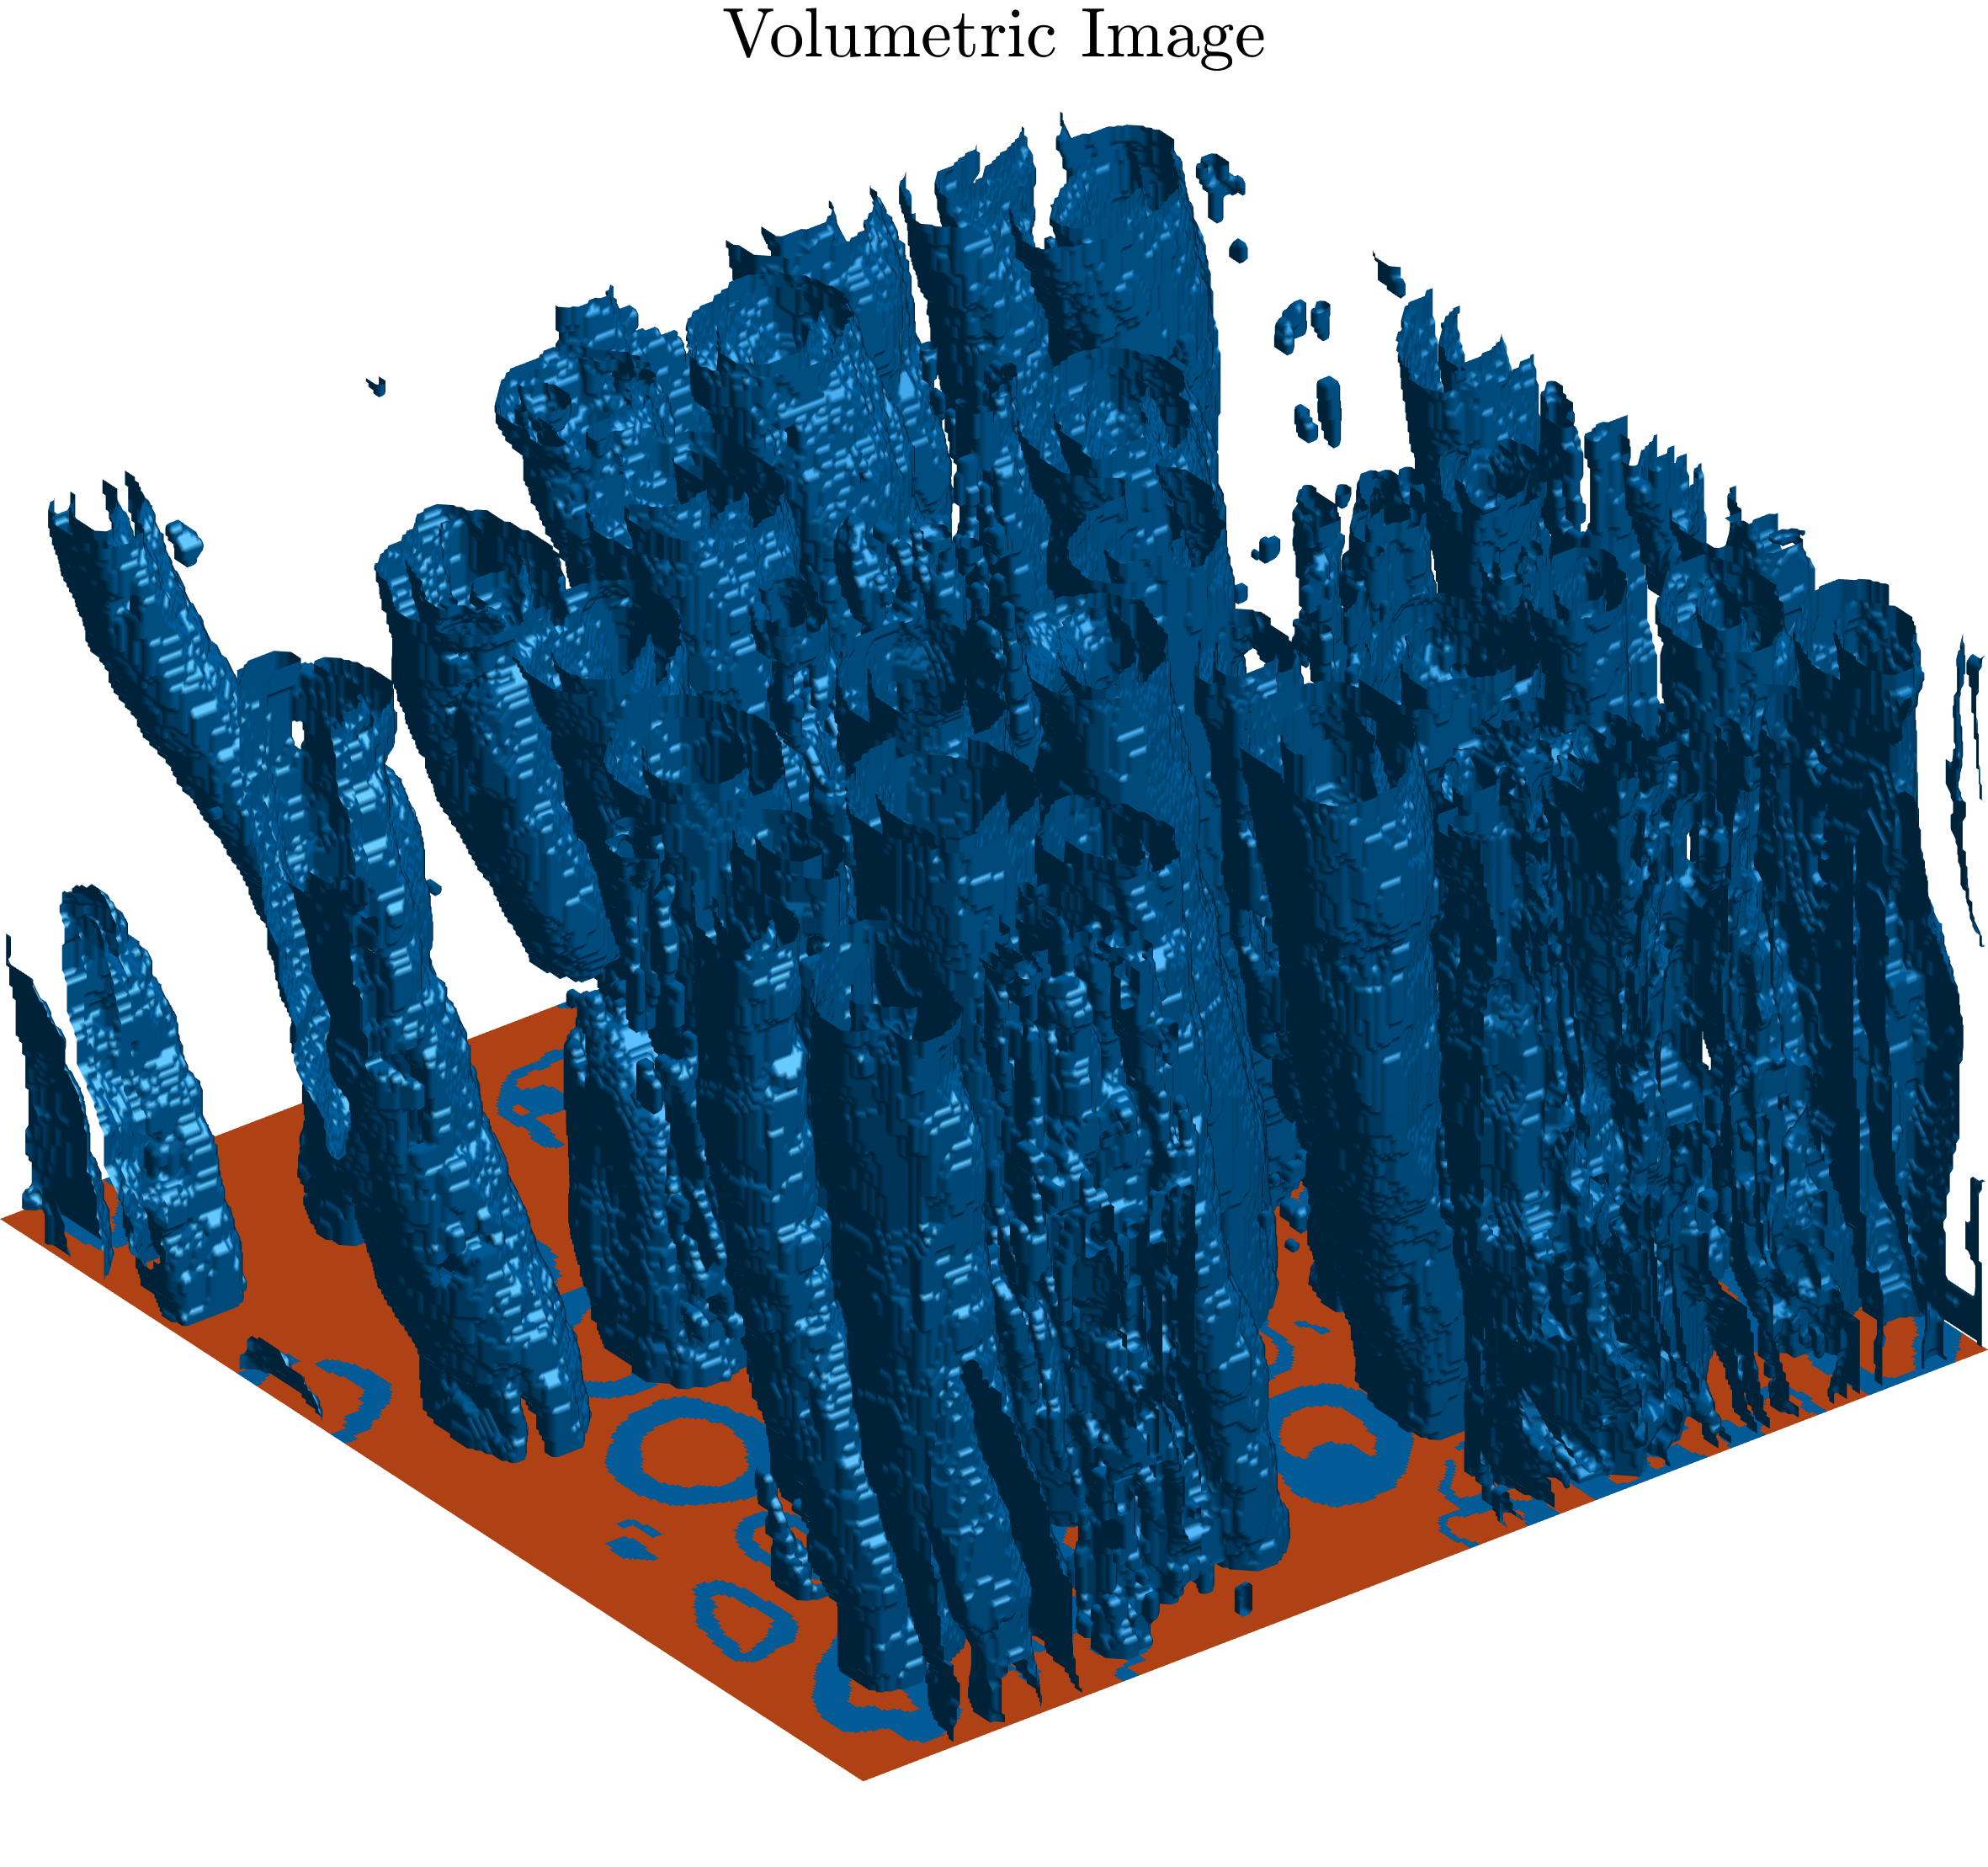
\includegraphics[width=0.8\textwidth]{./figures/final_res2.png}
    \caption{Top image is a snapshot of the $3$D MRF segmentation of nerves image. Bottom image shows the 3D visualization of the segmented nerves (using $1-300$ frames).}
\label{final2}
\end{figure}    

\item Perform deformable models using the Chan-Vese approach. Since a nerve consists of dark myelin and a bright axon, $m_{in}$ and $m_{out}$ have to be estimated from a thin band inside and outside the curve. In order to implement this modification without adding too many computational burdens, what I did here are as follows:
\begin{itemize}
    \item \textit{poly2mask}: find enclosed region of the curve, denoted as $mask_1$;
\item \textit{findboudary}: self-implemented function for finding boundary of the mask given by a certain curve;
\item \textit{imdilate}: extend the boundary to its neighbouring pixels by morphological operations, denoted as $mask_2$.
\item $m_{in}$ and $m_{out}$ can be easily computed by taking the mean intensities of pixels covered by $mask_1\ \&\ mask_2$ and $xor(mask_1\ \&\ mask_2, mask_2)$.
\item Combination of MRF and deformable models: use MRF to do the binary segmentation, then two options were tried:
\begin{itemize}
	\item[*] Apply deformable models on the segmented binary image.
	\item[*] Use binary image as a mask and crop patches from the original image.
\end{itemize}
    Finally, the Chan-Vese approach is applied to the processed image.
\end{itemize}
A snapshot of the final result is shown in Figure~\ref{final3}.
	\begin{figure}[!b]
	\centering
	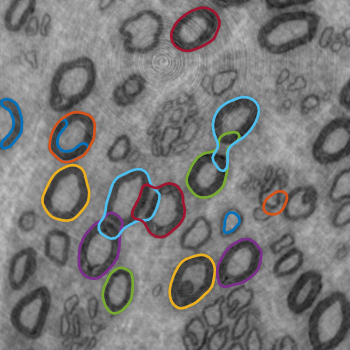
\includegraphics[width=0.5\textwidth]{./figures/257.png}
	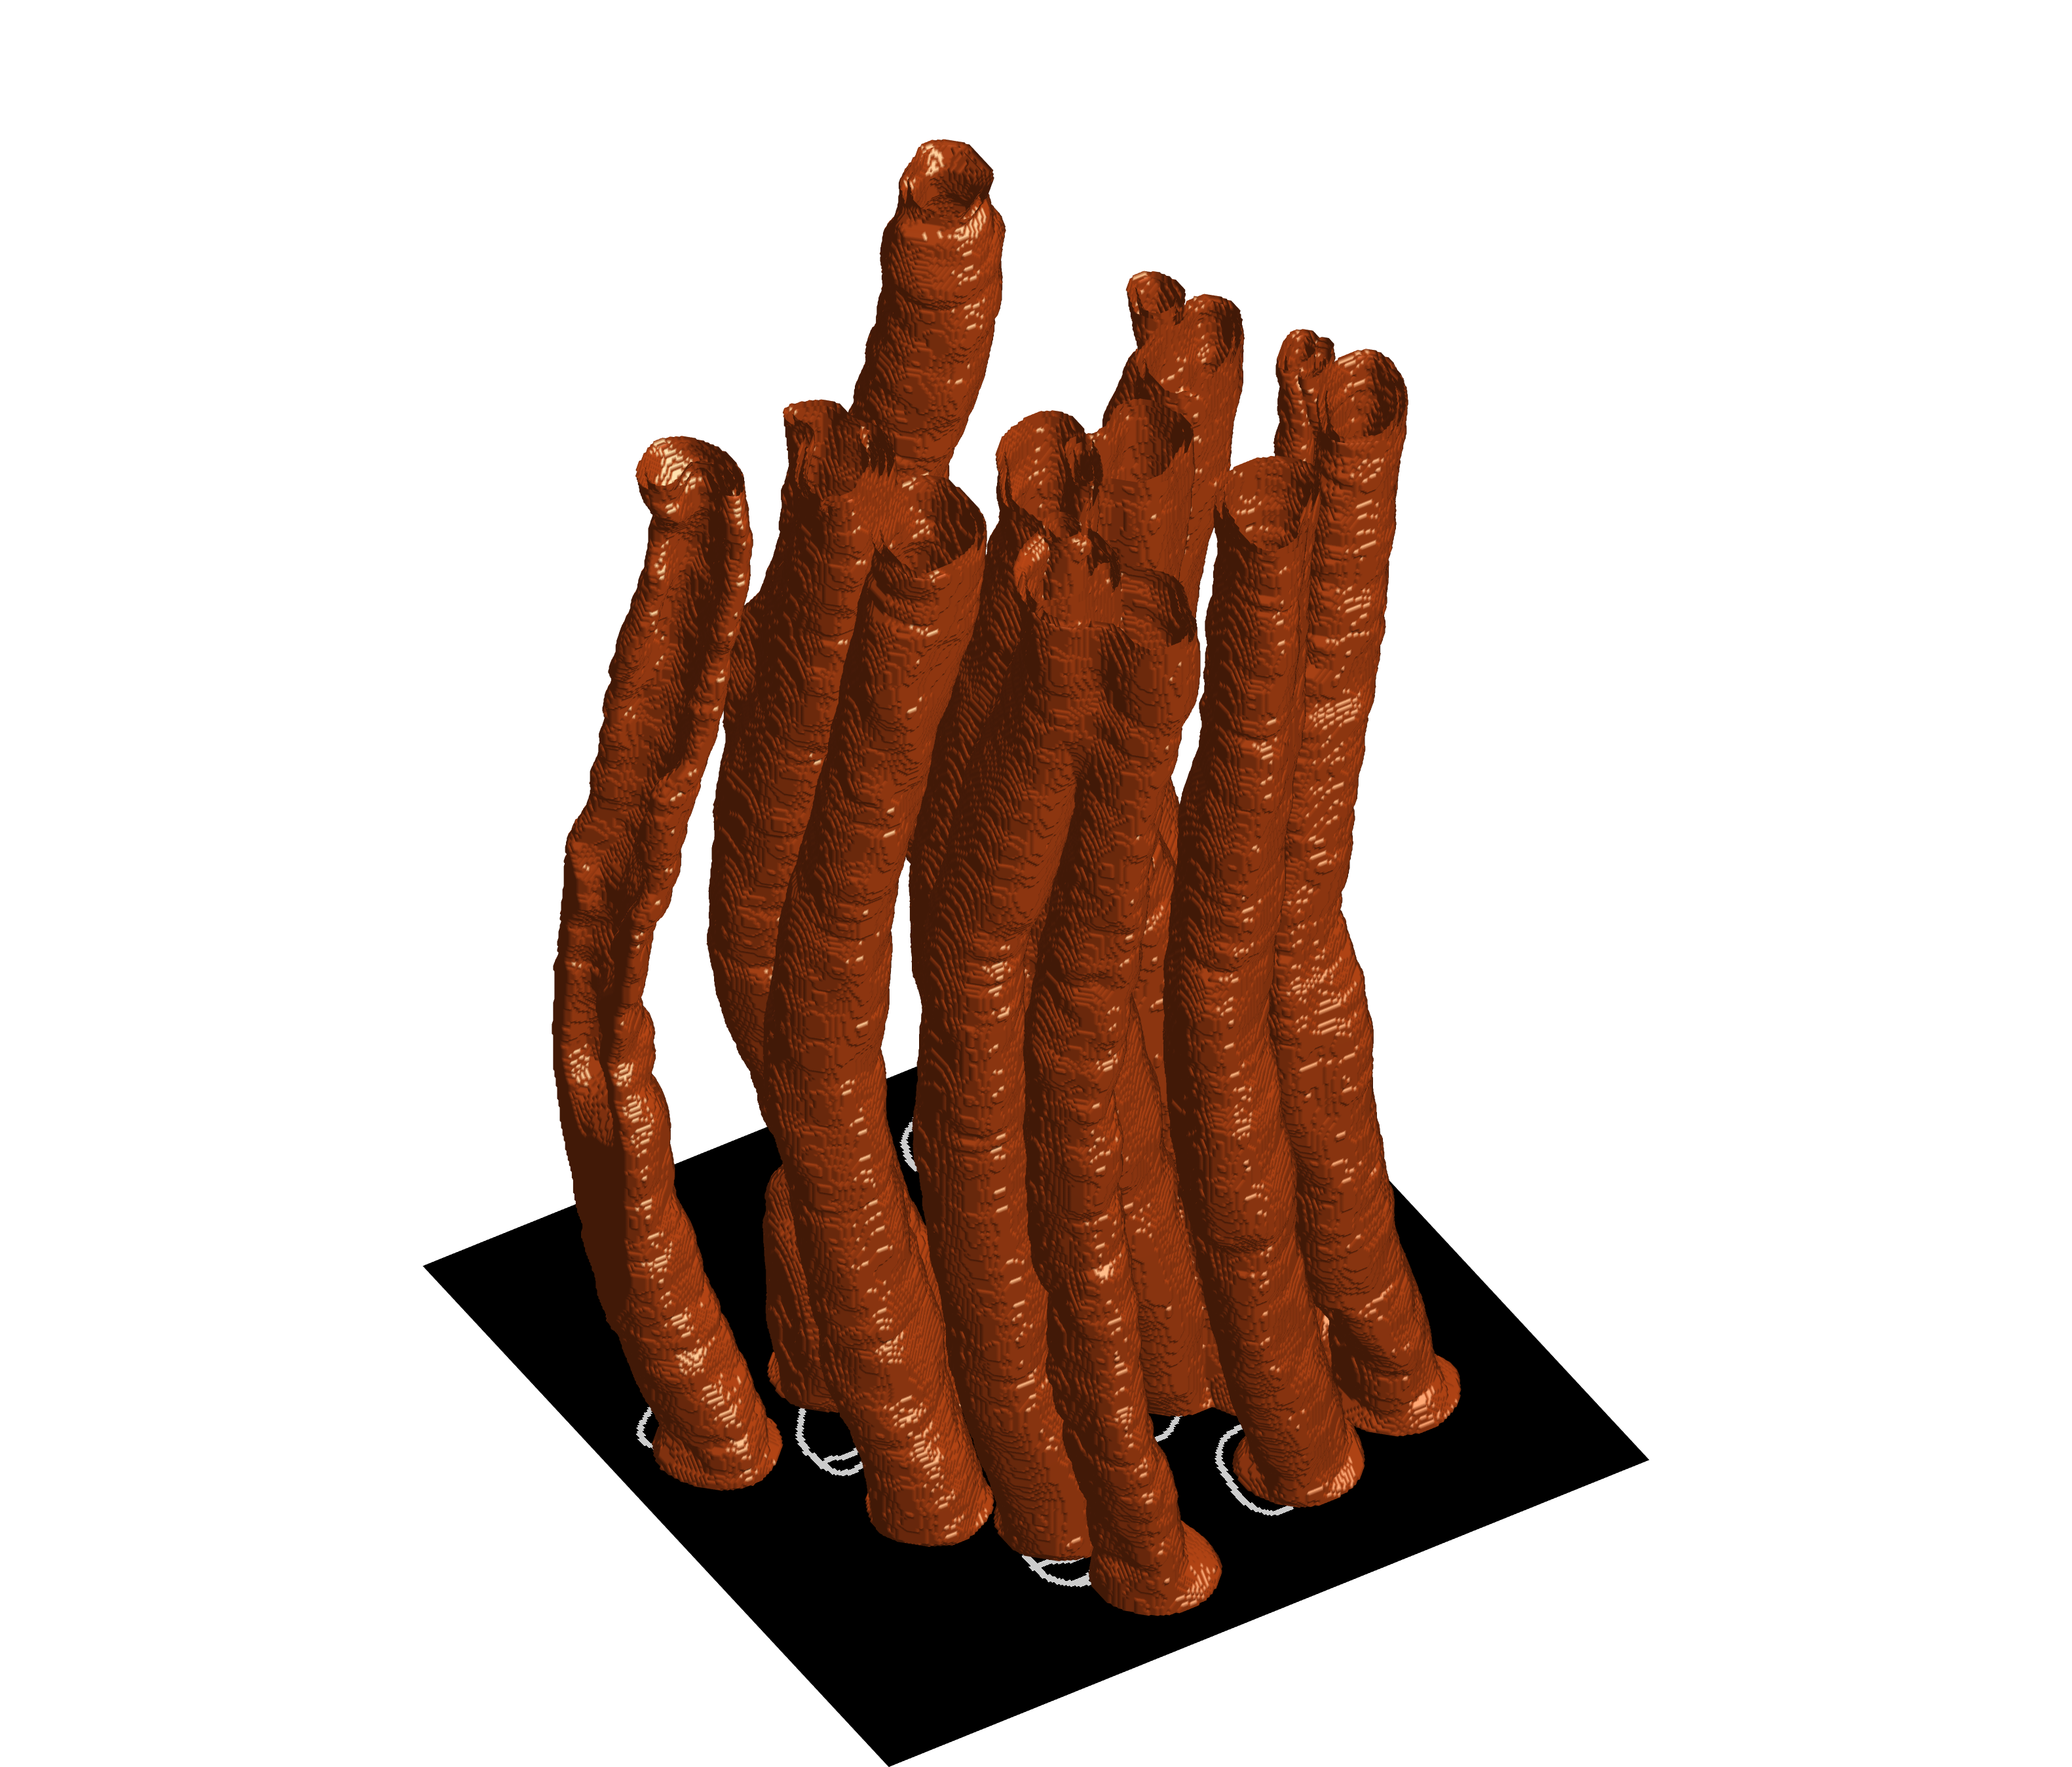
\includegraphics[width=0.8\textwidth]{./figures/final_res3.png}
    \caption{Top image is a snapshot of the segmentation of nerves image using the Chan-Vese approach. The bottom image shows the 3D visualization of the segmented nerves (using $1-500$ frames).}
	\label{final3}
\end{figure}		

\section{Discussion}
    From these results, some observations can be obtained:
\begin{itemize}
	\item Deformable model based approach can generate more fine segmentation while the results from MRF are more coarse. Moreover, $3$D full MRF produce a finer result than slice-by-slice based MRF. This is easy to understand since the curve is continuously tracked which means frame-to-frame (or temporal) information is considered. Similarly, $3$D full MRF also considers frame-to-frame smoothness priors. As a result, they can produce better results than the single frame based MRF. 
	\item Although the Chan-Vese method provides finer segmentation result, MRF is more efficient than the Chan-Vese method. Apparently, the complexity of the Chan-Vese method grows linearly with the curves involved. 
\end{itemize}
Some possible improvements:
	\begin{itemize}
		\item For both methods, images with significant contrast can make the segmentation easier and more stable. So it is always a good idea to generate images of good quality.
		\item For both methods, parameter tuning plays a key role in their performance. However, tuning is tedious work for human being. Perhaps reinforcement learning can be used to automatically tune those parameters.
		\item More efficient combination of the two methods. The following are some thoughts:
		\begin{enumerate}
			\item Since MRF is very fast but produces coarse results, we can use MRF not for binary segmentation, but for intensity enhancement (like estimating disparity for stereo vision system). For example, MRF will give a high intensity to pixels with a high probability of being background but a low intensity to pixels of nerves. Then we use Chan-Vese to get the fine result. Compared the two experiments carried out in the second assignment (assignment deformable models), it is clear that "Crawling Amoeba" experiment shows better performance because the foreground is more salient in "Crawling Amoeba" dataset. So although the result from MRF is coarse, if it can make the contrast between foreground and background more clear, it can definitely help the Chan-Vese approach.
			\item The geometric model (circle or ellipse) of nerves can be used as a penalty to constrain the shape of the curves and avoid cross-intersection between two close objects. As can be seen in those results, two close objects may pull the curve of the other to the wrong side. I think the ordinary shape of the curve can serve as a prior to suppressing this problem.
			\item MRF can also benefit from the Chan-Vese method. We can use the Chan-Vese curves to dynamically adjust or automatically tune the mean intensities used for computing likelihood in MRF.
		\end{enumerate}
	\end{itemize}		
	\end{enumerate}		
	
%https://youtu.be/KMWywGcNNjI	
%https://youtu.be/_GslxUDEZzM
	
	%\bibliography{PnPCites} 
	%\bibliographystyle{ieeetr}
	
\end{document}